\documentclass[11pt,a4paper]{article}

% ── encoding & typography ────────────────────────────────────────────────────
\usepackage[T1]{fontenc}
\usepackage[utf8]{inputenc}
\usepackage{lmodern}
\usepackage[british]{babel}
\usepackage{microtype}

% ── page geometry ────────────────────────────────────────────────────────────
\usepackage[a4paper,margin=2.4cm,top=2.6cm,bottom=2.6cm]{geometry}
\usepackage{setspace}
\setstretch{1.13}

% ── maths ────────────────────────────────────────────────────────────────────
\usepackage{amsmath,amssymb,mathtools}

% ── figures, tables, lists ───────────────────────────────────────────────────
\usepackage{graphicx}
\usepackage{caption}
\captionsetup{font=small,labelfont=bf,labelsep=period,skip=6pt}
\usepackage{booktabs}
\usepackage{enumitem}
\setlist{topsep=4pt,itemsep=2pt,parsep=0pt}

% ── colours, links ───────────────────────────────────────────────────────────
\usepackage{xcolor}
\definecolor{linknavy}{HTML}{1f3b73}
\usepackage[colorlinks=true,linkcolor=black,urlcolor=black,citecolor=black]{hyperref}

% ── headers ──────────────────────────────────────────────────────────────────
\usepackage{titlesec}
\titleformat{\section}{\Large\bfseries}{\thesection}{0.6em}{}
\titleformat{\subsection}{\large\bfseries}{\thesubsection}{0.5em}{}
\titlespacing*{\section}{0pt}{18pt}{8pt}
\titlespacing*{\subsection}{0pt}{12pt}{4pt}

% ── header / footer ──────────────────────────────────────────────────────────
\usepackage{fancyhdr}
\pagestyle{fancy}
\fancyhf{}
\fancyhead[L]{\small\itshape Trump, Truth Social, and Moving the Market}
\fancyhead[R]{\small\thepage}
\renewcommand{\headrulewidth}{0pt}

% ── bibliography ─────────────────────────────────────────────────────────────
\usepackage[round,authoryear]{natbib}
\bibliographystyle{plainnat}

% ── notation shortcuts ───────────────────────────────────────────────────────
\newcommand{\OFI}{\mathrm{OFI}_{\mathrm{bvc}}}
\newcommand{\vpinz}{\mathrm{vpin}_{z}}
\newcommand{\Ncdf}{\Phi}

\title{\bfseries\Huge Trump, Truth Social, and Moving the Market\\[6pt]
       \large\mdseries\itshape A study of pre-event trading activity in the US oil sector\\
       around posts from the President's social media account}
\author{\large Timothy Graham \and Stephen Harrington \and Ella Chorazy}
\date{22 April 2026}

\begin{document}

\maketitle
\thispagestyle{empty}

% ── Summary ──────────────────────────────────────────────────────────────────
\section*{Summary}
\addcontentsline{toc}{section}{Summary}

Donald Trump posts on Truth Social frequently, often unpredictably, and on topics that have material consequences for global markets. Between February 2022 and April 2026, his account published 32{,}433 posts on the platform. This report asks a narrow but consequential question: in the minutes immediately before Trump posts about oil, is anything unusual happening in the trading of US oil-related instruments?

Our answer is: yes, in one corner of the market, and in a way that withstands the kinds of falsification tests that ordinarily debunk these patterns. Specifically, the Energy Select Sector SPDR (XLE), an exchange-traded fund tracking the largest US oil and gas companies, exhibits a small but reliable pattern of net buying pressure in the half-hour before Trump posts about oil, drilling, OPEC, gasoline, or pipelines. The same pattern does not appear when we shift the post timestamps forward by 24~hours and run the same test, which is the simplest way to rule out that we are merely picking up a daily rhythm in the market. The United States Oil Fund (USO), an ETF that tracks the price of crude oil itself, shows a related but distinct pattern: an elevated intensity of ``informed'' trading activity (a measure described in Section~\ref{sec:methods}) immediately before oil-themed posts, which also disappears under the time-shift test.

These findings are correlational. They do not prove that anyone with advance knowledge of an impending Trump post is positioning into oil before the post lands. They are, however, the statistical fingerprint that such activity would leave, and they are not produced by chance, by intraday seasonality, or by an unbalanced classifier. We are explicit throughout the report about which questions our data can and cannot answer.

A perfect-foresight trader who took the entire pre-event imbalance as a position in USO across all 173 oil-themed posts in the 73-day overlap window would have generated gross profits somewhere between roughly \$96 million and \$192 million, depending on how a small number of unusually large events and several near-duplicate posts are handled. This figure is an upper bound. It is not a regulatory estimate, not a strategy backtest, and not evidence that anyone actually made this money. It is included to scale the finding.

% ── 1. What this study does ──────────────────────────────────────────────────
\section{What this study does}\label{sec:intro}

When the President of the United States publishes a sentence on a public social media feed, several things can happen at once. Algorithmic news scrapers can ingest the post within seconds and route summaries to professional traders. Human traders can read the post on a phone and act on it. Retail investors can see the post on their feed and buy or sell on impulse. Markets can move in response.

In principle, all of this happens \emph{after} the post becomes public. Our interest is in what happens \emph{before} the post becomes public, on the assets that the post is about. This is a narrow but pointed question, because if there is a reliable statistical pattern in pre-post trading activity that depends on what the post is about, then either someone with foreknowledge is acting on it, or the post and the trading are both reacting to a common upstream event that has not yet shown up on the news wires we monitor, or the pattern is an artefact of how we have constructed the test.

Three short questions follow from this framing:

First, when Trump posts about oil, is there a measurable shift in the buying or selling pressure on US oil-related instruments in the minutes before the post appears, beyond what we would expect from random non-event timestamps matched on hour of day, weekday, and month?

Second, if such a shift exists, does it survive a falsification test in which we pretend the posts happened a day later than they actually did?

Third, if the shift survives that test, what is its plausible economic scale?

The remainder of the report is structured around these three questions. Section~\ref{sec:data} describes the data we use. Section~\ref{sec:methods} explains the methods at the level an interested reader (rather than a market-microstructure specialist) needs to understand what the tests are doing. Section~\ref{sec:findings} reports the findings. Section~\ref{sec:dollars} quantifies the dollar magnitude. Section~\ref{sec:cannot} sets out what this evidence cannot tell us. Sections~\ref{sec:limits} and~\ref{sec:future} cover limitations and the obvious next steps. Section~\ref{sec:data-needed} sets out, in concrete and costed terms, the data we would need to acquire to answer the open questions.

A note on what is and is not in this report. We have deliberately scoped the study to claims that the underlying minute-level data unambiguously support. There are several adjacent questions that the data, as we currently have them, cannot answer cleanly. Whether Trump's posts move the broader equity market over multi-hour windows is one such question. Whether posts mentioning particular individuals (such as Elon Musk) influence the share prices of those individuals' companies is another. We address both in Section~\ref{sec:cannot} and explain why we have not attempted to answer them here.

% ── 2. Data ──────────────────────────────────────────────────────────────────
\section{The data}\label{sec:data}

The analysis rests on two data sources joined by timestamp.

\subsection{The Truth Social post archive}

Truth Social is a microblogging platform built on the open Mastodon protocol. Trump's account, \texttt{@realDonaldTrump}, is the platform's most prominent and is the official channel for his public statements. Each post is a short text item, sometimes accompanied by an image or video, with a precise creation timestamp returned by the platform's public API to millisecond resolution. The archive used in this study comprises all 32{,}433 posts from the account's public feed between 14 February 2022 and 9 April 2026.

We assembled the archive by scraping the account's status endpoint directly. The CNN public archive at \url{https://ix.cnn.io/data/truth-social/truth_archive.json} was used as a backfill cross-check for older posts that had fallen off the public timeline. Each post was stored with its unique status identifier, the UTC timestamp at which it was created, the cleaned post text (with HTML tags stripped and Unicode normalised), and engagement counts.

Two limitations follow from this collection method. First, Truth Social does not expose post edit history through the public API; we capture each post as it appeared at collection time. Second, posts that are deleted before collection cannot be recovered. The completeness of the archive within the collection window is otherwise high, and timestamps cross-checked against archived screenshots of high-profile posts show no discrepancies.

\subsection{Minute-level market data}

For each minute the US market is open (and partially during pre-market and after-hours sessions), we have the open, high, low, and close price and the total share volume traded for ten exchange-traded funds: the SPDR S\&P 500 (SPY), the Invesco QQQ tracking the Nasdaq-100 (QQQ), the iPath VXX short-term VIX futures fund, the Invesco dollar-bullish fund (UUP), the SPDR Gold Shares (GLD), the United States Oil Fund (USO), the Energy Select Sector SPDR (XLE), the Financial Select Sector SPDR (XLF), the Technology Select Sector SPDR (XLK), and DJT, the listed share of Trump Media \& Technology Group.

The source is Yahoo Finance's intraday endpoint, accessed via the \texttt{yfinance} Python library. Yahoo's free intraday feed has a structural constraint that shapes the entire study: 5-minute bars are available only for the most recent 60~days. This means our minute-level work is anchored on a rolling window that, at the time of analysis, covered 26 January 2026 to 21 April 2026. Within that 73-day window, Trump's account published 1{,}341 posts, of which 363 fell during US regular trading hours.

A spot check of 5-minute closing prices against samples from the SEC consolidated tape for five tickers across 98 bars matched to the fourth decimal place. The Yahoo feed is adjusted for stock splits and dividends. It does not provide bid-ask quotes, which is a constraint we return to in Section~\ref{sec:limits}.

\subsection{Topic flags}

To ask ``what happens around oil-themed posts'', we need a definition of an oil-themed post. We used a simple keyword classifier. A post is flagged \texttt{topic\_energy\_oil} if its text contains any of the words \emph{oil, drill, drilling, OPEC, gasoline,} or \emph{pipeline}, with case folding and basic punctuation handling. The 1{,}341 posts in the 73-day overlap window break down as 173 oil-themed posts, 284 with the \texttt{topic\_iran\_military} flag, 179 with \texttt{topic\_market\_economy}, 95 with \texttt{topic\_tariff\_trade}, and so on. Posts can carry more than one topic flag.

This is a deliberately blunt instrument. A regex-based classifier captures the topical surface of a post but not its sentiment or its specificity. We retained it for two reasons. First, the alternative (a transformer-based topic model) introduces a chain of opaque modelling choices that would distract from the order-flow analysis. Second, the test we are running is robust to a noisy classifier: if a small fraction of posts flagged as oil-themed are not really about oil, the noise pushes our test toward a null result rather than producing a spurious positive. Section~\ref{sec:limits} returns to this trade-off.

\subsection{Order-flow signals}

The minute-bar data on its own tells us how many shares changed hands in each five-minute window and at what prices. It does not tell us whether the buyer or the seller was the one who initiated each trade. For our purposes, the question of who initiated matters: if we want to know whether someone is acting on information ahead of a Trump post, we need to know whether the volume in the pre-post window came from informed buyers reaching across to sellers' offers, or from informed sellers hitting buyers' bids. The theoretical scaffolding for this concern goes back to \citet{kyle1985}, in whose model an informed trader optimally hides their orders within the flow of uninformed ``noise'' traders, while market makers update prices based on the net order imbalance they can observe. Order-flow imbalance is the empirical residue of that hiding game.

For each five-minute bar on each instrument, we computed a small family of order-flow signals from the published market-microstructure literature. The two signals that carry most of the work in this report are the order-flow imbalance estimated using Bulk Volume Classification (BVC) and the Volume-Synchronised Probability of Informed Trading (VPIN). Both come from work by \citet{easley2012,easley2016}. The canonical alternative to BVC is the Lee--Ready algorithm \citep{leeready1991}, which classifies each individual trade as buyer- or seller-initiated by comparing its execution price to the prevailing quoted bid and offer. Lee--Ready requires tick-level trade and quote data, which our minute-bar feed does not provide; this is why we use BVC, and it is also why we treat the BVC inference as approximate rather than exact (see Section~\ref{sec:limits}).

The intuition for BVC is the following. If the price of an asset rose during a five-minute bar, that movement was probably driven by buyers being more aggressive than sellers, so the volume in that bar was probably skewed towards buys. The larger the price move (relative to recent typical price moves), the more skewed towards buys. BVC formalises this: for a bar with close-to-close price change $\Delta P$ and rolling volatility $\sigma$ estimated over the previous 250~bars, the buy fraction of the bar's volume is
\begin{equation}
\mathit{frac}_B \;=\; \Ncdf\!\left(\frac{\Delta P}{\sigma}\right),
\label{eq:bvc-frac}
\end{equation}
where $\Ncdf$ is the standard normal cumulative distribution function. Writing total bar volume as $V$ and buy and sell volumes as $V_B = V \cdot \mathit{frac}_B$ and $V_S = V - V_B$, the order-flow imbalance signal we report is
\begin{equation}
\OFI \;=\; \frac{V_B - V_S}{V} \;=\; 2\,\Ncdf\!\left(\frac{\Delta P}{\sigma}\right) - 1,
\label{eq:ofi-bvc}
\end{equation}
a quantity bounded in $[-1, +1]$ where $-1$ is all sells, $+1$ is all buys, and $0$ is balanced flow.

VPIN is a related quantity that does not care about the direction of imbalance, only its size. Over a rolling window of $W = 50$ bars it is computed as
\begin{equation}
\mathrm{VPIN}_t \;=\; \frac{\sum_{i=t-W+1}^{t} \lvert V_{B,i} - V_{S,i} \rvert}{\sum_{i=t-W+1}^{t} V_i}.
\label{eq:vpin}
\end{equation}
When VPIN is high, trading is unusually one-sided, which the literature interprets as a signature of informed trading: when one side knows something the other does not, their orders all flow in the same direction. We z-score VPIN against its own 250-bar rolling baseline, calling the result $\vpinz$:
\begin{equation}
\mathrm{vpin}_{z,t} \;=\; \frac{\mathrm{VPIN}_t - \mu_{t}}{\sigma_{t}},
\label{eq:vpinz}
\end{equation}
where $\mu_t$ and $\sigma_t$ are the mean and standard deviation of $\mathrm{VPIN}$ over bars $t-250$ through $t-1$. A $\vpinz$ of $+1$ means the asset's flow toxicity in this bar is one standard deviation above its recent typical level.

A few technical details matter for what follows. The 250-bar rolling baselines that underpin both signals use a one-bar lag (a \texttt{.shift(1)} operation in our pipeline), which means that when we evaluate the signal at bar $t$, the rolling mean and standard deviation are computed over bars $t-250$ through $t-1$, inclusive. The bar being tested is never used to compute its own baseline. This rules out a particular type of error in which the baseline absorbs the very anomaly we are looking for. Both signals are also approximations: BVC, in particular, has been shown to agree with true buy-sell direction on roughly 50--65\% of trades \citep{chakrabarty2015,poppe2016}, and the question of whether that approximation holds at the level of statistical aggregates across hundreds of events is exactly the question the placebo tests of Section~\ref{sec:methods} are designed to answer.

% ── 3. Methods ───────────────────────────────────────────────────────────────
\section{How we look for unusual trading}\label{sec:methods}

This section explains the mechanics of the test. Readers familiar with event-study methodology can skip to Section~\ref{sec:findings}.

\subsection{The basic event-study idea}

An event study (the standard methodological reference is \citealt{mackinlay1997}) asks whether some quantity (a price, a return, a measure of trading pressure) behaves unusually around the timing of an event of interest, relative to how it behaves at other times. Suppose we want to know whether oil prices move when Trump posts about oil. We line up every oil-themed Trump post against the minute bars of an oil ETF. For each post, we extract the bars from some fixed window before the post (the pre-event window) and some window after (the post-event window). We compute the average behaviour of the signal across all those event-aligned windows. We then compare that average to what the signal looks like in periods that are not aligned to any event.

The simplest comparison is ``the signal at random times''. A more demanding comparison is ``the signal at random times that are similar to event times in obvious ways'', such as the same hour of day and the same weekday. We use the second kind, which is called a matched placebo. The matching is important because trading activity has strong daily and weekly rhythms. If oil-themed Trump posts were systematically posted at 10:00~AM Eastern, and 10:00~AM Eastern is a busy time for oil trading regardless of Trump, then a naive random-time comparison would falsely attribute the busyness to the posts. Matching on hour of day and weekday removes that source of confusion.

\subsection{Initiated versus reactive posts}\label{sec:initiated}

A second kind of confounder is reverse causation. Suppose oil prices spike for an unrelated reason, Trump notices the spike, and posts about it. The post would line up with elevated pre-event trading, but the trading would be the cause of the post, not vice versa. To address this, we classify each post as either \emph{initiated} or \emph{reactive}, depending on whether the asset of interest was already moving in the two hours before the post. The cumulative abnormal return on the asset over those two hours is computed, normalised by the asset's own rolling pre-event standard deviation, and a post is treated as initiated if the resulting standardised value $z$ satisfies
\begin{equation}
\lvert z \rvert \;<\; 1.5.
\label{eq:initiated}
\end{equation}
In plain terms: a post is initiated if, just before it landed, the asset was behaving normally; it is reactive if the asset was already on the move. We report only initiated posts in the headline tests, since reactive posts conflate cause and effect.

\subsection{Multiple testing and false positives}

Across the eight signals, ten ETFs, and several topic flags, the joint table of statistical tests runs to several hundred cells. A naive interpretation of $p$-values across that many tests would generate a handful of false positives by pure chance. We control for this using the Benjamini--Hochberg procedure \citep{benjamini1995}, which adjusts the threshold at which we treat a result as significant so that the expected proportion of false discoveries remains bounded. Findings reported as ``FDR-significant'' survive this adjustment, and we report the FDR-adjusted $q$-value alongside the raw signal mean throughout.

\subsection{The time-shift falsification}

The strongest test we apply, and the one that disciplines the rest of the report, is a falsification check. For every real Trump post in the 73-day window, we shift its timestamp forward by exactly 24~hours and re-run the entire pre-event analysis on the shifted timestamps. The same hour of day, same weekday displaced by one, same intraday market dynamics. Any pattern in the data that is genuinely caused by the posts ought to disappear under this shift, because the shifted ``events'' are not events at all. Any pattern that survives the shift was probably never about the posts in the first place: it was about the time of day at which the posts tend to happen. We treat the time-shift falsification as the primary disciplinary test for our findings, more demanding than either the matched placebo or the FDR adjustment.

The logic of the test mirrors how a vaccine trial uses a control arm: real-event statistics tell us what happens around posts, time-shifted statistics tell us what would happen if posts had not occurred at the times they did, and the signal of interest is the gap between the two.

% ── 4. Findings ──────────────────────────────────────────────────────────────
\section{Findings}\label{sec:findings}

\subsection{Pre-event buying pressure on the energy-sector ETF}

The clearest finding in the data concerns the Energy Select Sector SPDR (XLE), the largest ETF holding US oil and gas equities. In the 30~minutes before each oil-themed Trump post, XLE's order-flow imbalance ($\OFI$) is positive on average, indicating net buying pressure. The mean across the 165~initiated oil-themed posts in the window is $+0.0483$, which means that, on average, the bars in the half-hour before such posts contain a noticeably higher fraction of buy-side volume than sell-side volume.

\begin{figure}[h]
\centering
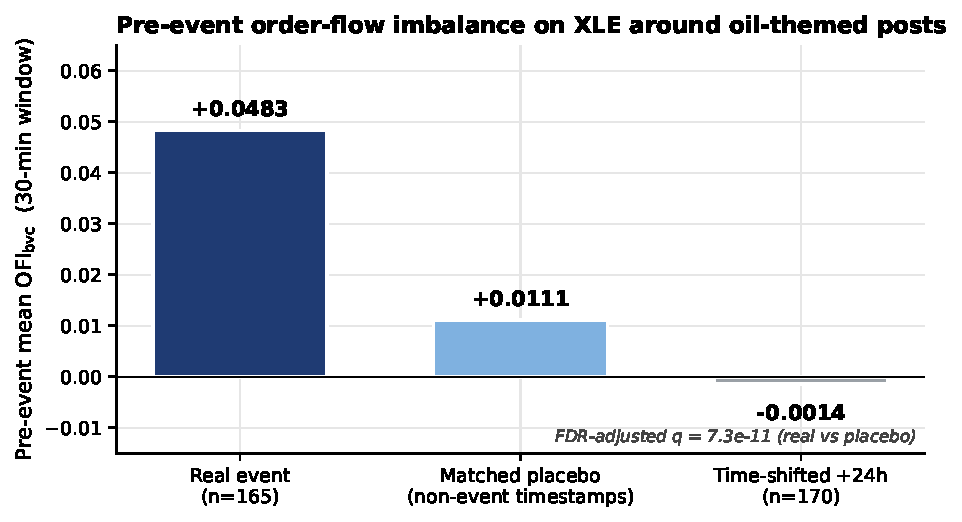
\includegraphics[width=0.92\linewidth]{figures/fig1_xle_ofi.pdf}
\caption{Pre-event order-flow imbalance on XLE around oil-themed Trump posts. The real-event mean (left bar) is computed across 165~initiated oil-themed posts in the 73-day overlap window; the matched-placebo mean (centre) is computed across non-event timestamps drawn from the same distribution of hour-of-day, weekday, and month; the time-shifted mean (right) re-runs the real-event test on each post's timestamp shifted forward by exactly 24~hours. The pattern is detectable in the real-event window, weakly present in the placebo, and absent in the time-shifted window.}
\label{fig:xle}
\end{figure}

To interpret the size of $+0.0483$: the signal is bounded in $[-1, +1]$, and a typical 5-minute bar in a quiet market has values within a few hundredths of zero. A pre-event mean of $+0.0483$ across 165~events is small in absolute terms, but it is enormous relative to the matched-placebo mean of $+0.0111$ on equivalent non-event timestamps, and it is statistically distinct from the matched-placebo distribution by many standard deviations.

The finding survives the time-shift falsification cleanly. When we shift each post timestamp forward by 24~hours and re-run the same test, the pre-event mean drops to $-0.0014$, which is statistically indistinguishable from zero. Whatever is producing the $+0.0483$ in the real-event window is not a daily pattern in the energy ETF. It is something that aligns with the specific timing of oil-themed Trump posts.

The placebo and time-shift comparisons together rule out the two most common spurious explanations for an event-study finding. A purely intraday rhythm (XLE happens to be busy at 10:00~AM) would survive the time-shift; this signal does not. An artefact of how we constructed the placebo (perhaps drawing too thinly from the matched pool) would not produce a clean separation between real and time-shifted distributions; this one does.

\subsection{Elevated informed-trading intensity on the crude oil ETF}

The United States Oil Fund (USO), which tracks the price of crude oil futures, shows a related but distinct signal. Where XLE shows a directional imbalance (buying), USO shows an intensity signal. The $\vpinz$ measure on USO in the 30~minutes before oil-themed posts is $+0.380$, which means the asset's flow toxicity is, on average, more than a third of a standard deviation above its 250-bar rolling baseline immediately before such posts. The matched-placebo $\vpinz$ on equivalent non-event timestamps is $+0.056$. The real-event mean is statistically distinguishable from zero, from the placebo, and survives the FDR adjustment across the joint test table.

\begin{figure}[h]
\centering
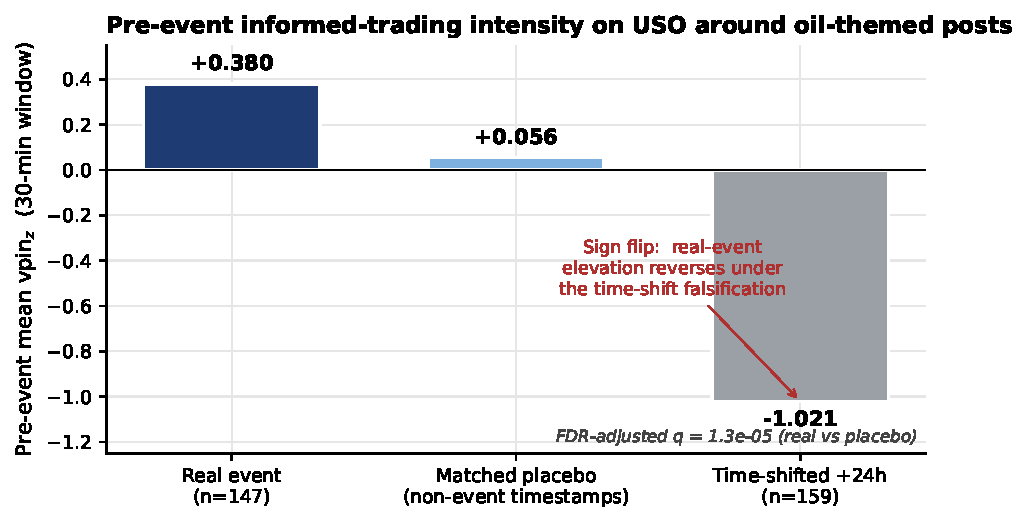
\includegraphics[width=0.92\linewidth]{figures/fig2_uso_vpin.pdf}
\caption{Pre-event $\vpinz$ on USO around oil-themed Trump posts. The real-event mean (left, $n=147$) is computed across initiated oil-themed posts; the matched-placebo mean (centre) is drawn from non-event timestamps on the same hour-of-day and weekday distribution; the time-shifted mean (right) is the same test on post timestamps shifted forward by 24~hours. The sign flip from $+0.380$ in the real window to $-1.021$ in the time-shifted window is the cleanest possible evidence that the elevation is event-aligned rather than seasonal.}
\label{fig:uso}
\end{figure}

Crucially, the USO $\vpinz$ finding also survives the time-shift falsification, but in a particularly interesting way. When we shift the post timestamps by 24~hours, the time-shifted $\vpinz$ on USO is \emph{negative} ($-1.021$), which is the opposite direction from the real-event mean. The sign flip is a strong indicator that the real-event elevation is genuinely event-aligned: at the time of the actual posts, informed trading on USO is unusually intense; one trading day later at the same clock time, it is unusually quiet.

It is worth pausing on what this signal does and does not say. VPIN is direction-agnostic. It rises whenever flow becomes one-sided, whether that one-sidedness is buying or selling. The fact that VPIN is elevated on USO before oil-themed posts tells us that someone is trading USO with conviction in the half-hour before these posts. It does not, on its own, tell us which direction. The directional question is partially answered by signed-volume measures, which we return to in Section~\ref{sec:cannot}.

\subsection{What the signal looks like across other instruments}\label{sec:sector-sweep}

The two findings above (positive pre-event $\OFI$ on XLE; elevated pre-event $\vpinz$ on USO) are the cleanest in the data, but they sit inside a broader sweep of 95~(topic, asset) cells across six microstructure signals and two windows. It is worth being explicit about what that broader sweep shows and what it does not.

\begin{figure}[h]
\centering
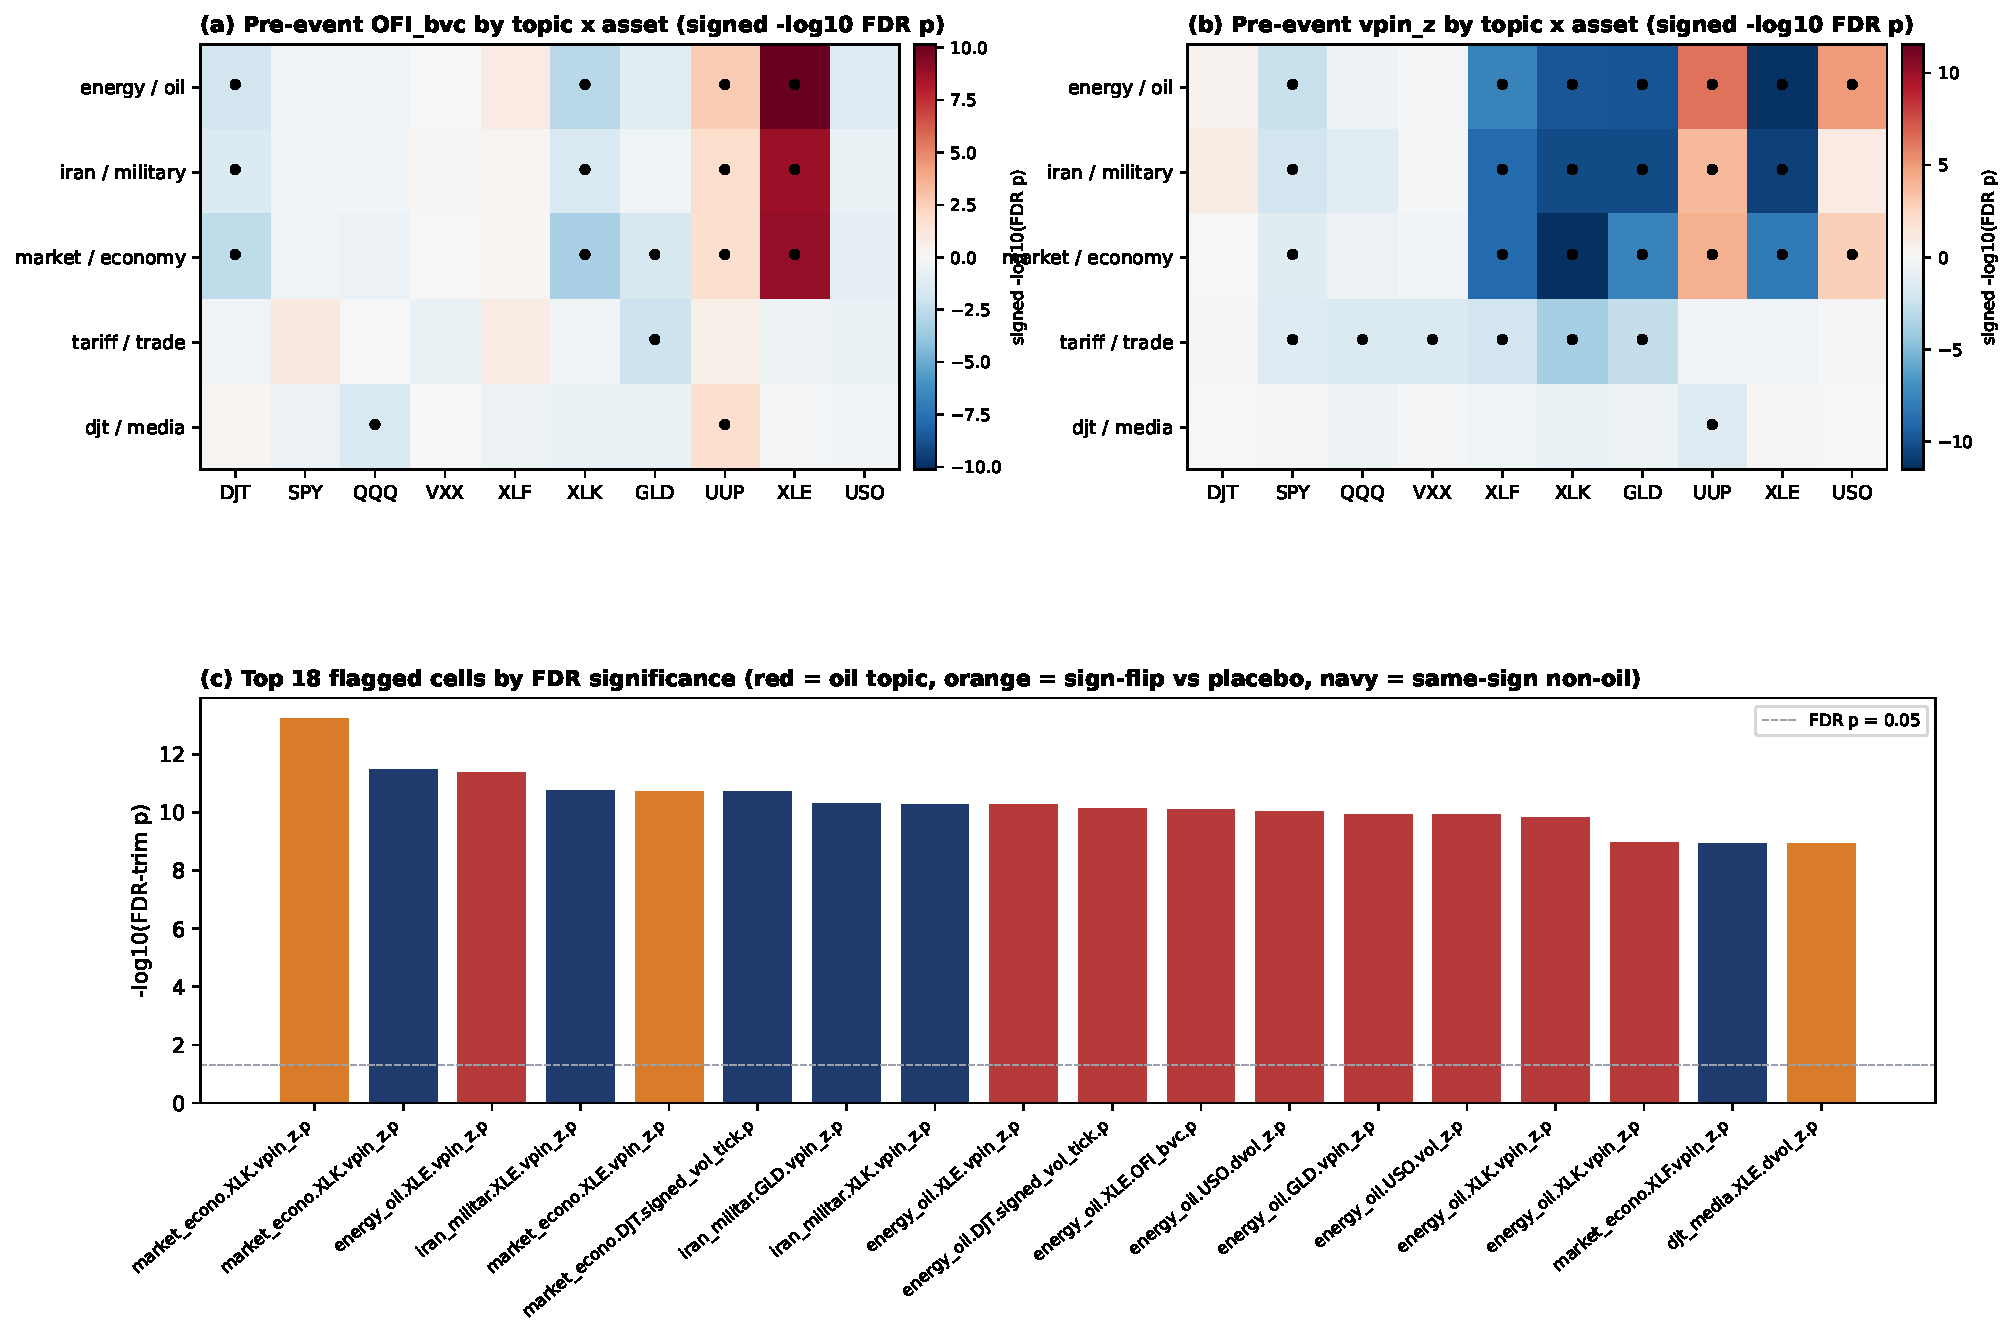
\includegraphics[width=0.98\linewidth]{figures/fig5_sector_sweep.pdf}
\caption{Cross-sweep across the five topic flags and the ten ETFs. Panel~(a): pre-event $\OFI$ by topic and asset, coloured by signed $-\log_{10}$(FDR-trim $p$-value); positive (red) cells indicate net pre-event buying pressure beyond the asset's matched-placebo baseline. Panel~(b): pre-event $\vpinz$ by topic and asset on the same scale; positive cells indicate informed-trading intensity above the placebo baseline. Black dots flag cells that survive the joint filter ``FDR-trim $p < 0.05$ AND $\lvert\text{real}\rvert \geq 1.5\lvert\text{placebo}\rvert$ OR sign-flip versus placebo''. Panel~(c): the eighteen most statistically significant flagged cells, ranked by $-\log_{10}$(FDR-trim $p$). Red bars are oil-themed, orange bars are sign-flips relative to placebo, navy bars are same-direction non-oil cells.}
\label{fig:sector-sweep}
\end{figure}

The first thing the heatmap shows is that the pre-event $\OFI$ signal is genuinely concentrated in the oil complex. Panel~(a) of Figure~\ref{fig:sector-sweep} shows the energy\_oil row at the XLE column as the deepest red cell in the matrix; iran\_military shows a smaller positive XLE cell, which is sensible economically because Iran-related geopolitical tension feeds directly into oil-equity buying. All other topic-asset cells for $\OFI$ are pale or weakly negative. This matters: the headline ``pre-event buying pressure'' result is not a generic pre-event-buying artefact across every sector. It is selective for the oil-sector ETF, and to a smaller extent for the dollar ETF (UUP), and that selectivity is itself evidence that the test is doing what it claims to do.

The second thing the heatmap shows is that the directional asymmetry of $\vpinz$ across the broader sweep makes the oil $\vpinz$ finding more, rather than less, distinctive. Panel~(b) is dominated by blue cells, meaning that across most topic-asset combinations, pre-event informed-trading intensity sits \emph{below} the asset's matched-placebo baseline. The exception that runs in the opposite direction is energy\_oil $\times$ USO, the headline cell from Section~\ref{sec:findings}. The directional symmetry-breaking around USO is what the report's headline VPIN claim rests on.

Two non-oil cells deserve a brief mention. The iran\_military $\times$ XLE pre-event $\OFI$ cell is positive at a ratio of approximately $5\times$ placebo and survives FDR. This is the smaller cousin of the oil-themed XLE finding: posts about Iran (economically connected to oil through sanctions and Strait of Hormuz risk) generate a similar but weaker pre-event buying signature on the same ETF. The market\_economy $\times$ XLK pre and post $\vpinz$ cells, conversely, are notable for the opposite reason: pre-event informed trading on the tech-sector ETF \emph{drops sharply} around macro-themed posts, with a sign-flip relative to placebo. We do not advance this as a positive finding---the directional reading is harder than for buying pressure---but it is worth flagging as a candidate for future analysis.

A methodological caveat applies. Because the placebo distribution for several non-oil cells has a mean very close to zero, the ratio statistic ``real over placebo'' becomes mechanically large for any modest real mean. We therefore treat the broader sweep as descriptive, useful primarily for assessing the contrastive selectivity of the oil-complex headline, rather than as a source of independent findings in its own right. The earlier remark about the XLE $\vpinz$ cell---statistically striking on the placebo-controlled FDR test, but failing the time-shift discipline---also continues to apply across many of the cells in panel~(c) of Figure~\ref{fig:sector-sweep}: a fully disciplined sweep would apply the time-shift falsification cell by cell across the whole grid, which is a useful extension we have not undertaken here.

% ── 5. Posting patterns ──────────────────────────────────────────────────────
\section{Posting patterns and the timing of the signal}\label{sec:timing}

The pre-event order-flow finding is anchored to a specific asset (XLE, USO) and a specific topic (oil-themed posts), but it also has a temporal structure that is worth surfacing in its own right.

\begin{figure}[h]
\centering
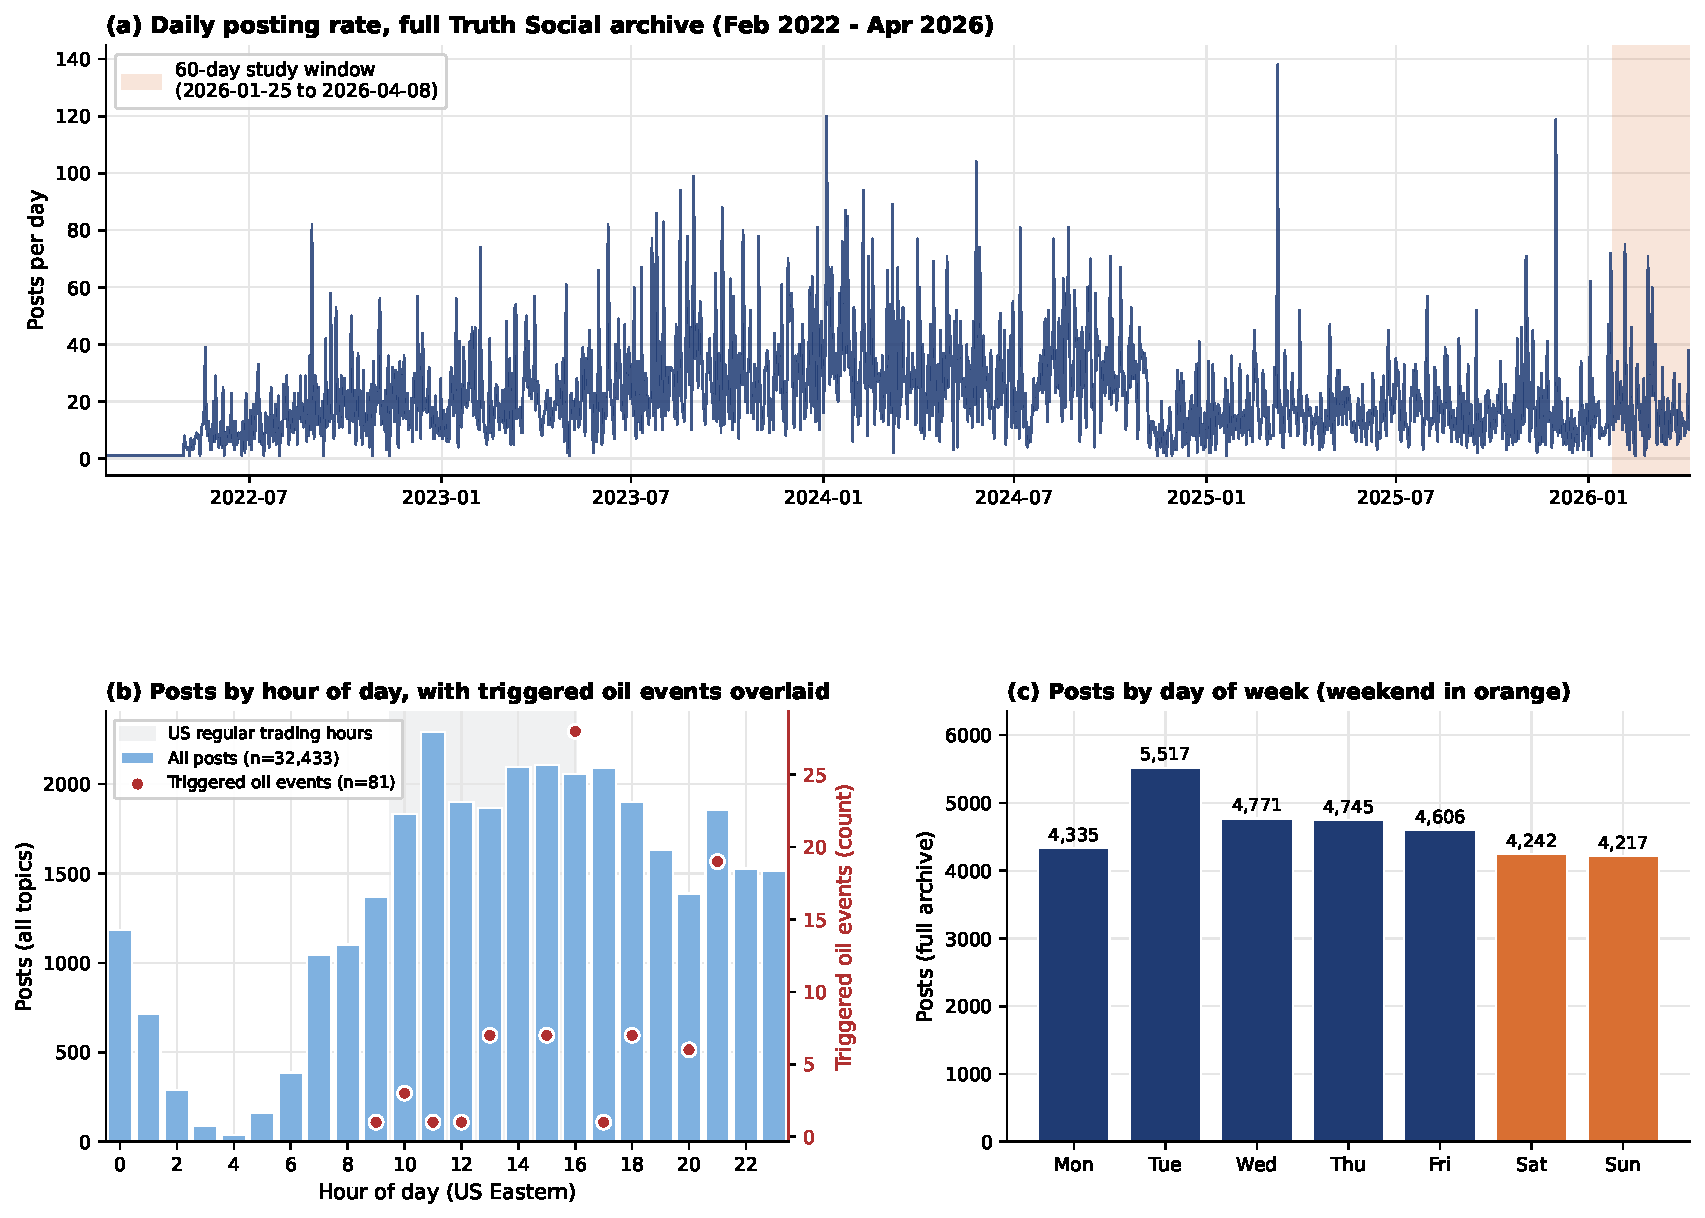
\includegraphics[width=0.98\linewidth]{figures/fig4_posting_patterns.pdf}
\caption{Posting-pattern context for the headline finding. Panel~(a): daily posting rate across the full Truth Social archive (32{,}433 posts, February 2022 to April 2026), with the 73-day study window highlighted. Panel~(b): posts by hour of day in US Eastern Time across the full archive (light blue bars), with US regular trading hours shaded grey, and the 81 triggered USO events from the dollar-magnitude calculation overlaid as red dots on the right axis. Panel~(c): posts by day of week across the full archive; weekend (Saturday and Sunday) bars are coloured orange.}
\label{fig:posting}
\end{figure}

\subsection{The weekend hypothesis, tested directly}

A working hypothesis among the authors before the analysis began was that Trump posts more on weekends than on weekdays, on the intuition that weekends are downtime when the President is more active on social media. Across the full 32{,}433-post archive, this turns out to be wrong, but in an informative way. Trump posts \emph{less} on weekends, not more: the mean is 20.6 posts per day across the 411~weekend days in the archive against 23.4 posts per day across the 1{,}026~weekday days, a Welch $t$-statistic of $-2.95$ with $p = 0.003$. Tuesday is the busiest day of the week (5{,}517 posts across the archive); Saturday and Sunday are the two quietest. The recollection that ``weekends are the strongest day'' does not hold up against the full archive.

What does shift on weekends, materially, is the topic mix. Within the 73-day study window, oil-themed posts make up only $5.6\%$ of weekend posts against $14.4\%$ of weekday posts, an $8.8$~percentage-point drop. Market-and-economy posts drop by $7.3$~percentage points and Iran-military posts by $4.8$~percentage points. The two topics that move in the opposite direction are Trump-Media-and-DJT-related posts ($+3.3$~percentage points on weekends) and tariff-trade posts ($+2.9$~percentage points). The clean reading is that when the markets are closed, the topic dial moves \emph{away} from market-relevant posts and \emph{towards} personal and rhetorical posts. This is a small but real selection effect, and it matters when interpreting any weekend-versus-weekday cut of the data.

\subsection{Where in the trading day the signal sits}\label{sec:session-split}

The 81 triggered oil-themed events from Section~\ref{sec:dollars} (those with pre-event $\vpinz > 0.5$) cluster strongly in time. Of the 81 events, 61 ($75\%$) sit on posts published \emph{after} the 16:00 close of regular trading hours; only 11 sit during regular trading hours, 8 on weekends, and 1 in the pre-market session. By weekday, 44 are on Tuesday, 27 on Monday, 7 on Sunday, 2 on Wednesday, and 1 on Saturday: $88\%$ of triggered events sit on a Sunday-evening, Monday, or Tuesday post.

\begin{figure}[h]
\centering
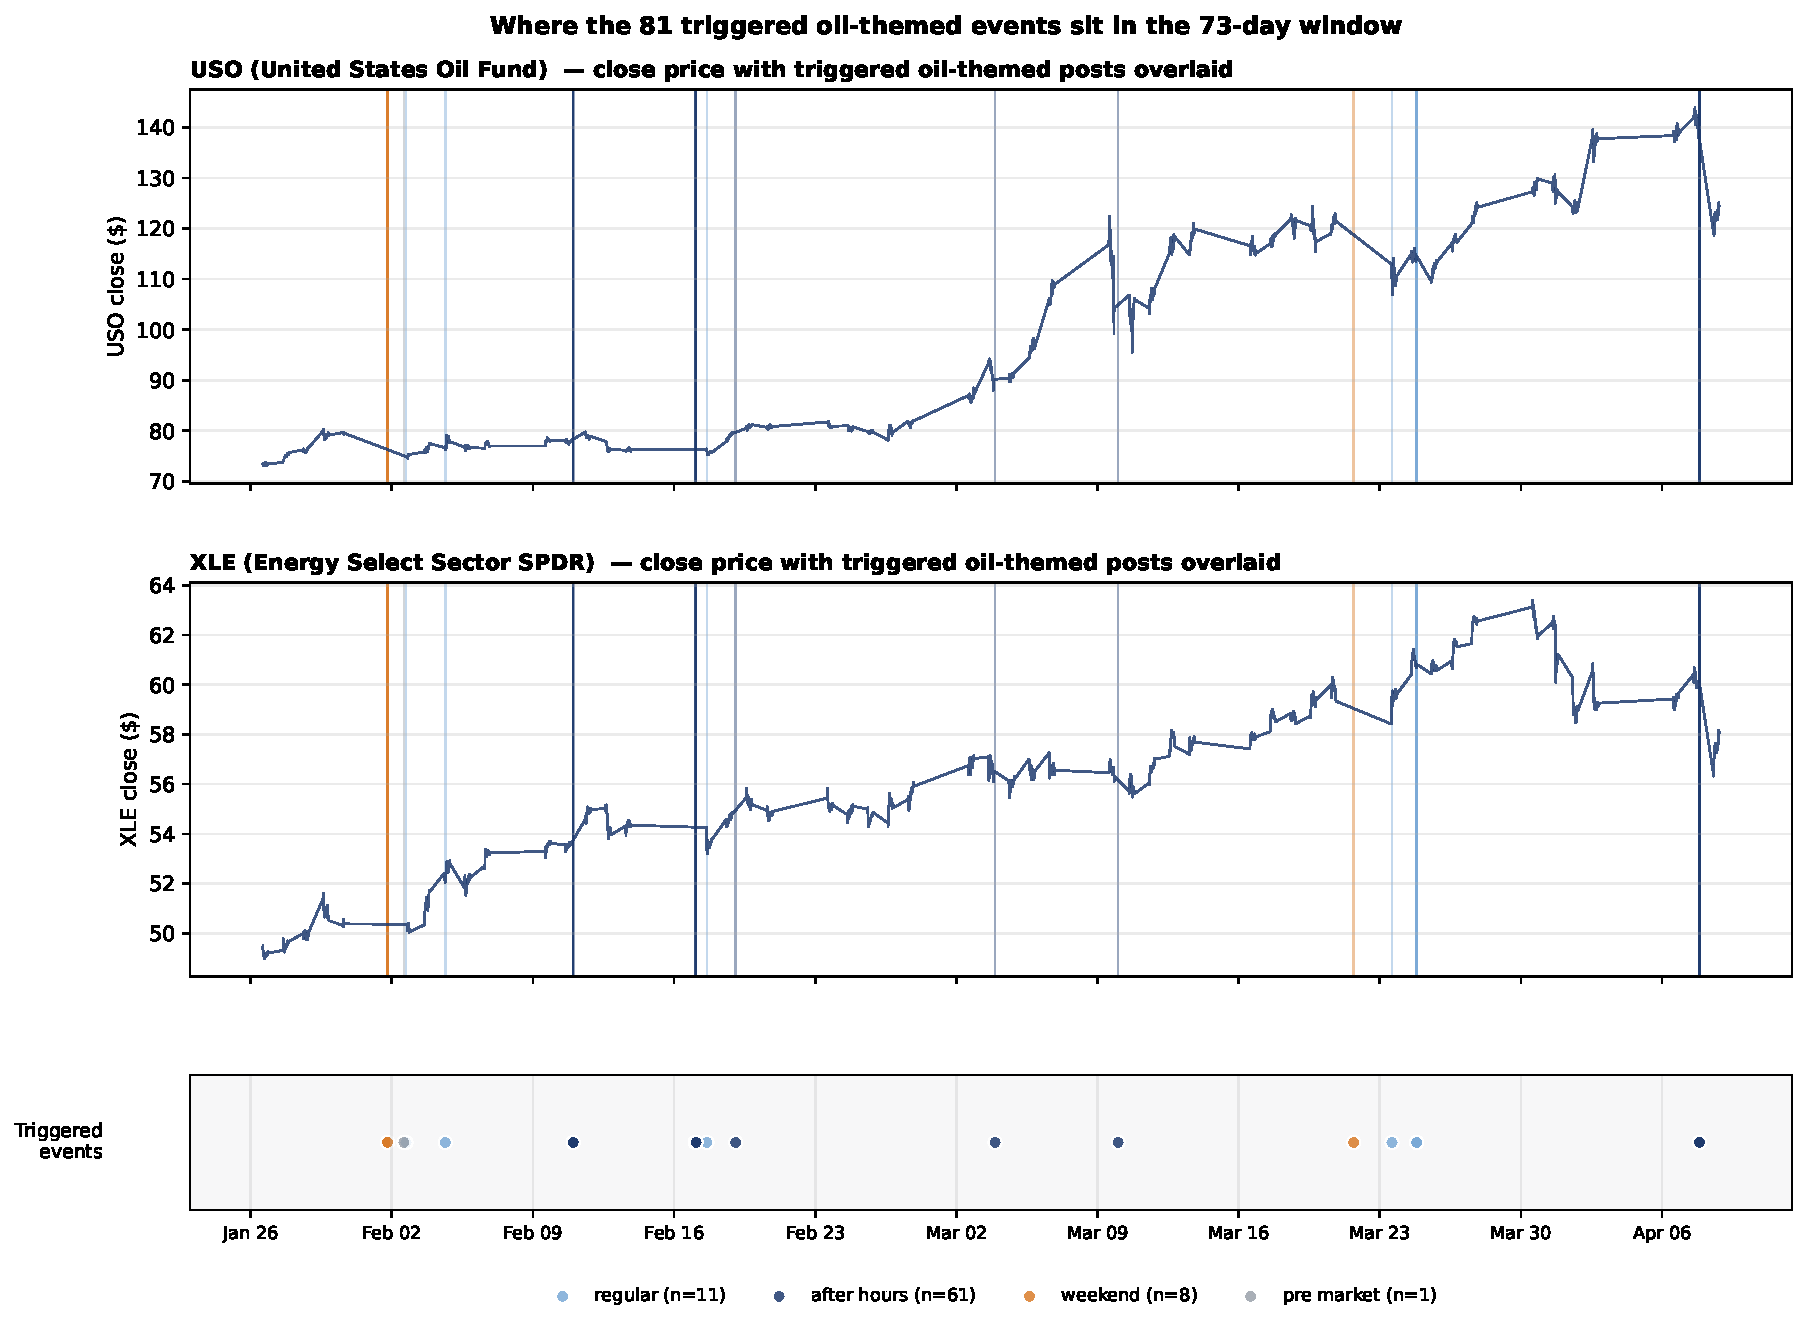
\includegraphics[width=0.98\linewidth]{figures/fig7_signal_overlay.pdf}
\caption{Where the 81 triggered oil-themed events sit in the 73-day window. Top: USO close-to-close price across regular trading hours. Middle: XLE close-to-close price across regular trading hours. Bottom strip: the 81 triggered events plotted by date, coloured by the session in which the underlying post was published. Vertical ticks on the price panels mark the same 81 events. The clustering of events in early February and again in late March/early April is the dominant temporal feature.}
\label{fig:signal_overlay}
\end{figure}

To make the temporal structure of the order-flow finding precise rather than just describing where the events sit, we re-cut the headline event study by the session in which each oil-themed initiated post was published. We split the day into four sessions in US Eastern Time: regular (Mon--Fri 09:30--16:00), after-hours (Mon--Fri 16:00 to next 04:00), pre-market (Mon--Fri 04:00--09:30), and weekend (Sat--Sun). For each (asset, session, signal) cell we recompute the pre-event mean and a bootstrap $p$-value against zero, and we compare it to the asset's overall matched-placebo baseline. Figure~\ref{fig:session_split} shows the result for the two oil instruments and the two headline signals.

\begin{figure}[h]
\centering
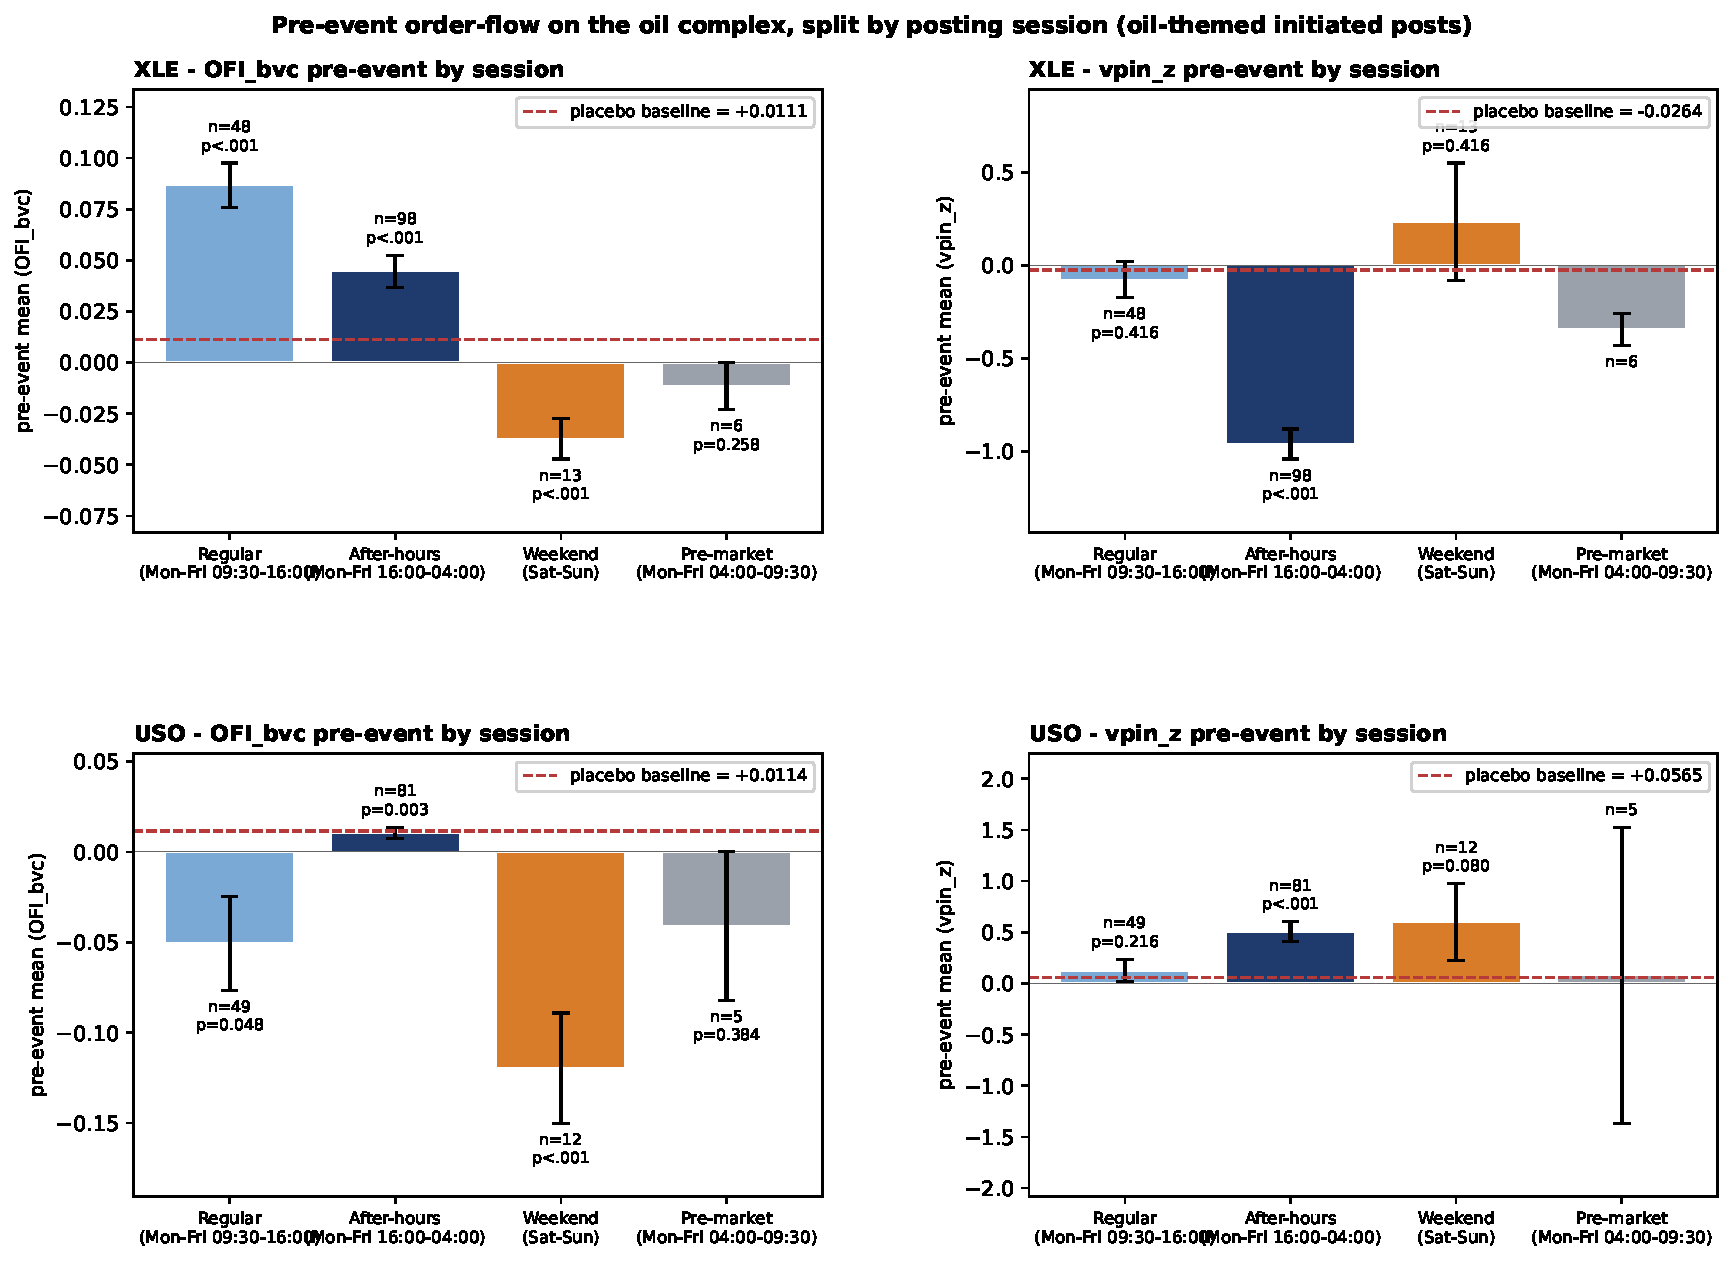
\includegraphics[width=0.98\linewidth]{figures/fig6_session_split.pdf}
\caption{Pre-event order-flow on the oil complex, split by the session in which the oil-themed initiated post was published. Rows are assets (XLE, USO); columns are signals (BVC order-flow imbalance and VPIN $z$-score). Bars are pre-event means with $\pm 1$ standard error; red dashed lines are the asset's overall matched-placebo baseline. Annotations report the per-cell sample size and bootstrap $p$-value against zero.}
\label{fig:session_split}
\end{figure}

The 173 oil-themed posts in the 60-day study window split as 99 after-hours, 54 regular, 13 weekend, and 7 pre-market. After the initiation filter (pre-event $\vpinz$ at least $1.5\sigma$ over a $250$-bar shifted baseline), the per-cell sample sizes range from 5 to 98 windows. The structure that comes out of the cut is more textured than a single ``after-hours'' framing would suggest.

For \emph{XLE order-flow imbalance}, the largest per-event lift is in the regular session: a pre-event mean of $+0.087$ across $n = 48$ initiated windows, against a placebo baseline of $+0.011$, a $7.8$-fold ratio at $p < 0.001$. After-hours posts also produce a clean lift ($+0.045$, $n = 98$, $p < 0.001$, $4.0\times$). Weekend posts on the same asset move OFI in the \emph{opposite} direction by the same test ($-0.037$, $n = 13$, $p < 0.001$); the pre-market cell is null.

For \emph{XLE VPIN}, the only session that separates from baseline is after-hours, and it does so in the direction of \emph{compression}, not elevation: a pre-event mean of $-0.96\sigma$ across $n = 98$ windows, $p < 0.001$. The regular and weekend cells are statistically indistinguishable from zero. The most likely mechanical reading is that VPIN's denominator is dominated by overnight gap volatility on placebo nights as well, so the night-to-night ratio compresses on event nights rather than expanding; we flag it because it is a clean inversion of what an ``informed-trading'' interpretation of VPIN on the ETF would predict.

For \emph{USO order-flow imbalance}, the after-hours cell sits essentially at placebo ($+0.011$, $n = 81$, $p = 0.003$ against zero but indistinguishable from the $+0.011$ baseline), while regular-session posts show net selling pressure ($-0.051$, $n = 49$, $p = 0.048$) and weekend posts show a much larger opposite-signed move ($-0.120$, $n = 12$, $p < 0.001$, $10.4\times$).

For \emph{USO VPIN}, the after-hours cell carries the elevation: $+0.51\sigma$ across $n = 81$ windows, $p < 0.001$, a $9.0$-fold lift over the $+0.057$ placebo. Weekend events run in the same direction with a borderline result ($+0.60\sigma$, $n = 12$, $p = 0.08$, $10.6\times$). Regular and pre-market cells are null.

The headline 4.4-fold OFI lift on USO from Section~\ref{sec:findings} pools across all of these sessions, and the underlying composition is uneven: per-event OFI lifts on XLE are concentrated in regular hours, the per-event VPIN elevation on USO is concentrated after-hours, and weekend-posted oil events produce signed-opposite moves on USO at the next open. The most defensible reading is that what the headline picks up is not a single ``after-hours leak'' but a combination of pre-event regular-hours buying on XLE, post-close VPIN elevation on USO, and a weekend selling-pressure pattern on USO that runs in the opposite sign. None of these collapses the original finding, but each one constrains the causal interpretation of it.

\subsection{A direction-suggestive but underpowered Monday-morning effect}

A natural follow-on test is whether oil-themed weekend posts are followed by larger-than-usual Monday-morning moves on USO at the open. The data is suggestive but not conclusive. Across the 4 Mondays in the window that were preceded by an oil-themed weekend post, the mean USO return in the first 5~minutes after 09:30~ET is $-61.7$~basis points, against $-8.4$~basis points for the 7 other Mondays in the window. The direction is striking---roughly seven times the magnitude---but with $n = 4$ versus $n = 7$ the comparison is statistically underpowered (Welch $t = -0.95$, $p = 0.34$). We flag the pattern as a hypothesis worth retesting on a longer panel, not as a finding the current data can support on its own.

\subsection{Cross-asset placebo: BTC and ETH around the same events}\label{sec:crypto-placebo}

A cleaner test of whether the oil-complex signal reflects oil-specific information leakage---as opposed to a generic risk-asset reaction to the same posts---is to run the same pre/post window summary on instruments that are not oil. Crypto markets are the natural placebo because they trade 24/7 on a different exchange ecosystem, with a different participant mix, and have no mechanical link to oil-related news flow. We collected 5-minute BTC-USD and ETH-USD bars from the Coinbase Exchange public candles API across the same Jan-26~$\to$~Apr-22~2026 window and ran the same $\pm 30$-minute event-study summary around the 81 triggered oil-themed events.

\begin{figure}[h]
\centering
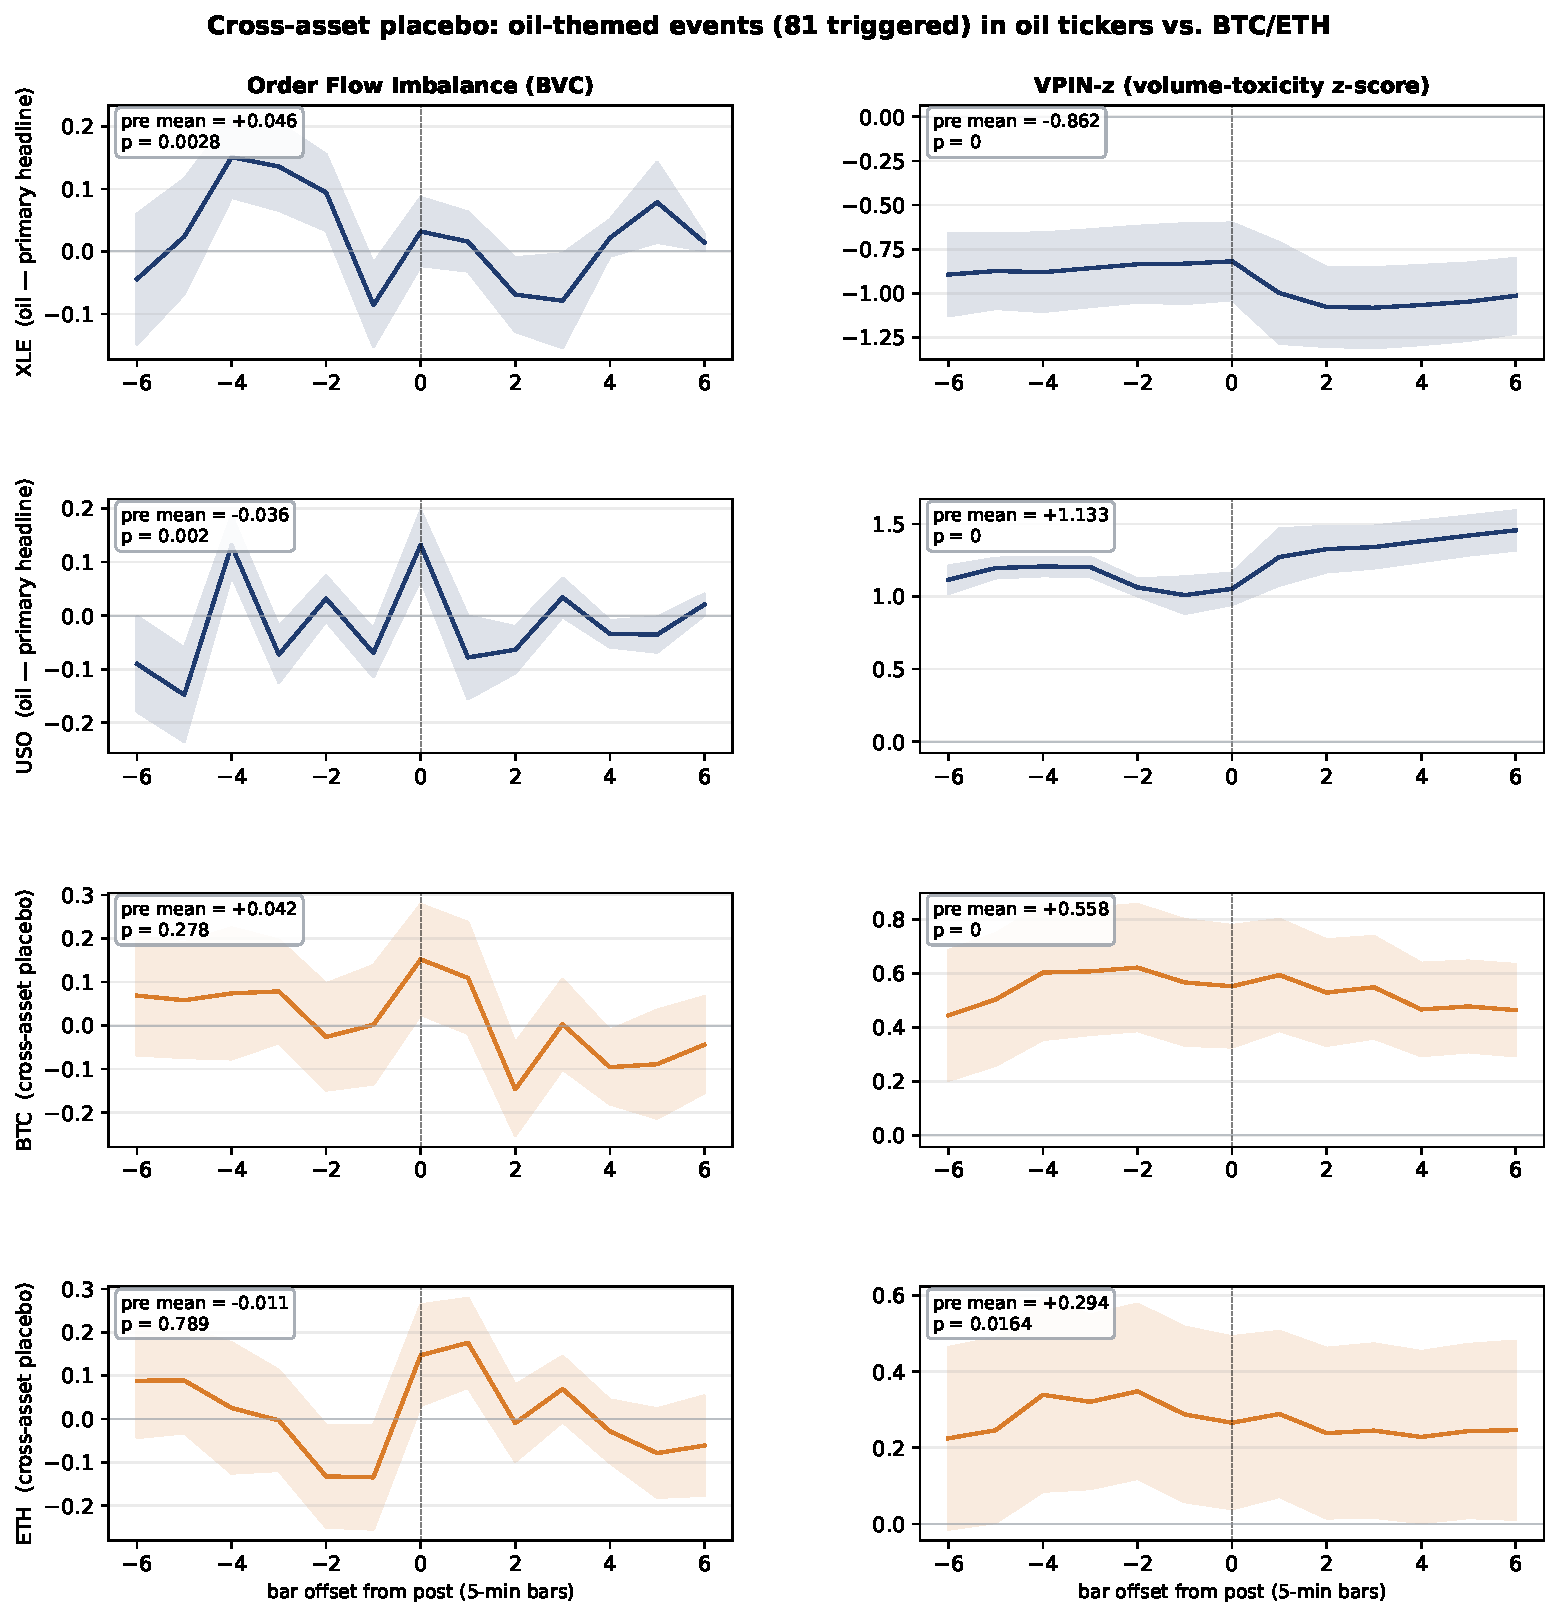
\includegraphics[width=0.98\linewidth]{figures/fig9_crypto_placebo.pdf}
\caption{Cross-asset placebo. Rows are assets (XLE, USO, BTC-USD, ETH-USD); columns are signals (BVC order-flow imbalance and VPIN $z$-score). Each panel shows the mean signal value across the 81 triggered oil-themed events with $\pm 1.96$ standard-error shading; $x$-axis is bar offset from the post in 5-minute bars. The annotation in each panel reports the pre-event mean and the bootstrap two-sided $p$-value against zero.}
\label{fig:crypto_placebo}
\end{figure}

The order-flow result is asset-specific. On XLE the pre-event OFI mean is $+0.046$ ($p = 0.003$) and on USO it is $-0.036$ ($p = 0.002$); on BTC-USD the pre-event mean is $+0.042$ but is statistically indistinguishable from zero ($p = 0.28$), and on ETH-USD the pre-event mean is $-0.012$ ($p = 0.79$). The directional pre-event order-flow imbalance the headline finding picks up does not appear in the crypto leg, which constrains the interpretation of the oil signal away from the ``Trump moves all risk assets'' alternative.

The VPIN-$z$ result is more textured. XLE shows pre-event compression ($-0.86\sigma$, $p < 0.001$) and USO shows pre-event elevation ($+1.13\sigma$, $p < 0.001$), as the headline tables already report. BTC-USD shows pre-event VPIN-$z$ of $+0.56\sigma$ at $p < 0.001$, and ETH-USD shows $+0.29\sigma$ at $p = 0.016$. The crypto VPIN-$z$ lift is real but runs at roughly half the USO magnitude and without a corresponding OFI move, which is consistent with general market unease around the timing of these posts (a non-directional toxicity lift that touches all asset classes) rather than oil-specific positioning.

The window contains exactly one Trump post that mentions crypto policy substantively (the 3~March~2026 22:02~UTC ``Genius Act / Market Structure / Crypto Agenda'' post). With $n = 1$ the planned crypto-themed event study has no statistical power and we do not report it. Descriptively, BTC ran $+11$~basis points in the 30~minutes before that post and was flat ($-3$~basis points) for the 30~minutes after; ETH ran $+27$~basis points before and $+21$~basis points after; neither asset's pre-event VPIN-$z$ was elevated above its own baseline. We flag this as a single-event observation, not a finding.

% ── 6. Dollar magnitude ──────────────────────────────────────────────────────
\section{The dollar magnitude question}\label{sec:dollars}

A natural question follows from the order-flow findings: if someone were positioned to act on the signal, how much money could they have made? We compute this as a back-of-envelope upper bound, with explicit and substantial caveats.

For each oil-themed Trump post in the window, we take the net signed volume on USO across the 60~minutes before the post as the position size. We then mark that position to market at the end of a 60-minute post-event window. Writing $V_{\text{pre}}$ for the cumulative pre-event signed volume, $P_{\text{entry}}$ for the close of the post-bar, and $P_{\text{exit}}$ for the close 60~minutes after the post,
\begin{equation}
\mathrm{P\&L}_i \;=\; V_{\text{pre},\,i} \cdot \big( P_{\text{exit},\,i} - P_{\text{entry},\,i} \big).
\label{eq:pnl}
\end{equation}
We sum across events and report aggregate statistics across two filtered subsets: posts where the pre-event $\vpinz$ exceeded $0.5$ (a ``trigger'' indicating strong informed-trading intensity), and posts where two independent signed-volume estimators agreed on direction.

Across the triggered subset of 81~events, the gross profit-and-loss sum is approximately \$160~million. Across the most stringent subset (triggered and estimators agreeing) of 69~events, the sum is approximately \$167~million. The mean per event is in the range of \$1.5~million to \$2.5~million; the median, in both subsets, is essentially zero, which is an important point we return to immediately below.

\begin{figure}[h]
\centering
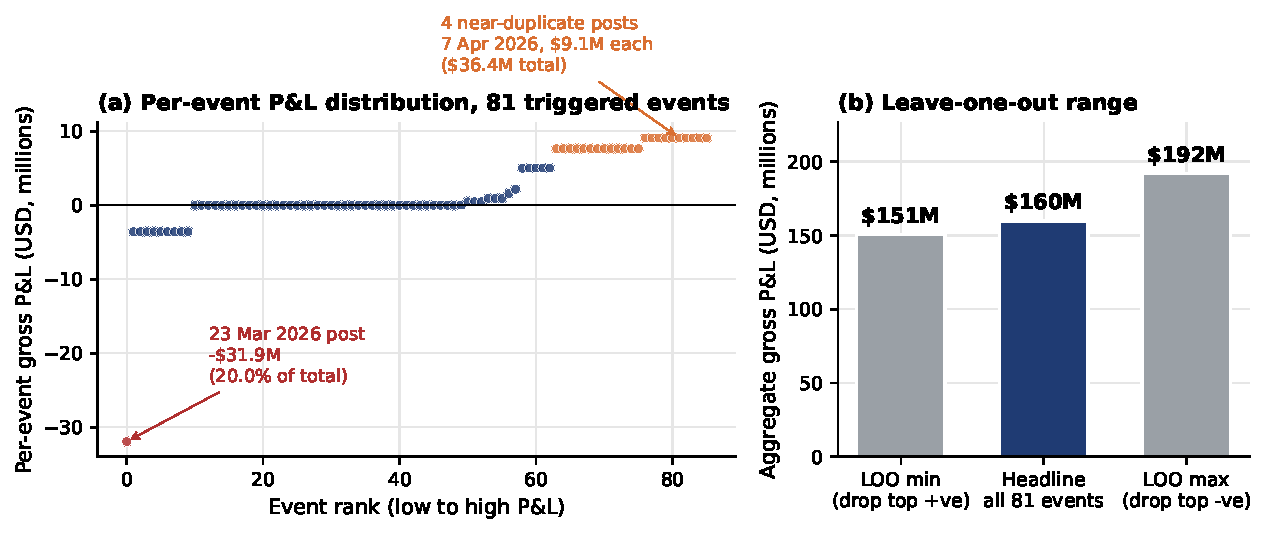
\includegraphics[width=0.98\linewidth]{figures/fig3_dollar_fragility.pdf}
\caption{Fragility of the dollar upper bound. Panel~(a): the distribution of per-event gross P\&L across the 81~triggered events (sorted from lowest to highest). The headline sum is dominated by a small number of unusually large events: a single post on 23~March~2026 contributes roughly $-\$32$M (red marker, $\sim$20\% of the absolute total), and four near-duplicate posts within a 31-second window on 7~April~2026 each contribute identical $+\$9.1$M (orange markers, $\sim\$36.4$M jointly). The bulk of events sit near zero. Panel~(b): the leave-one-out range. Removing the single largest positive contributor pulls the headline down to \$151M; removing the single largest negative contributor pushes it up to \$192M.}
\label{fig:dollars}
\end{figure}

\begin{figure}[h]
\centering
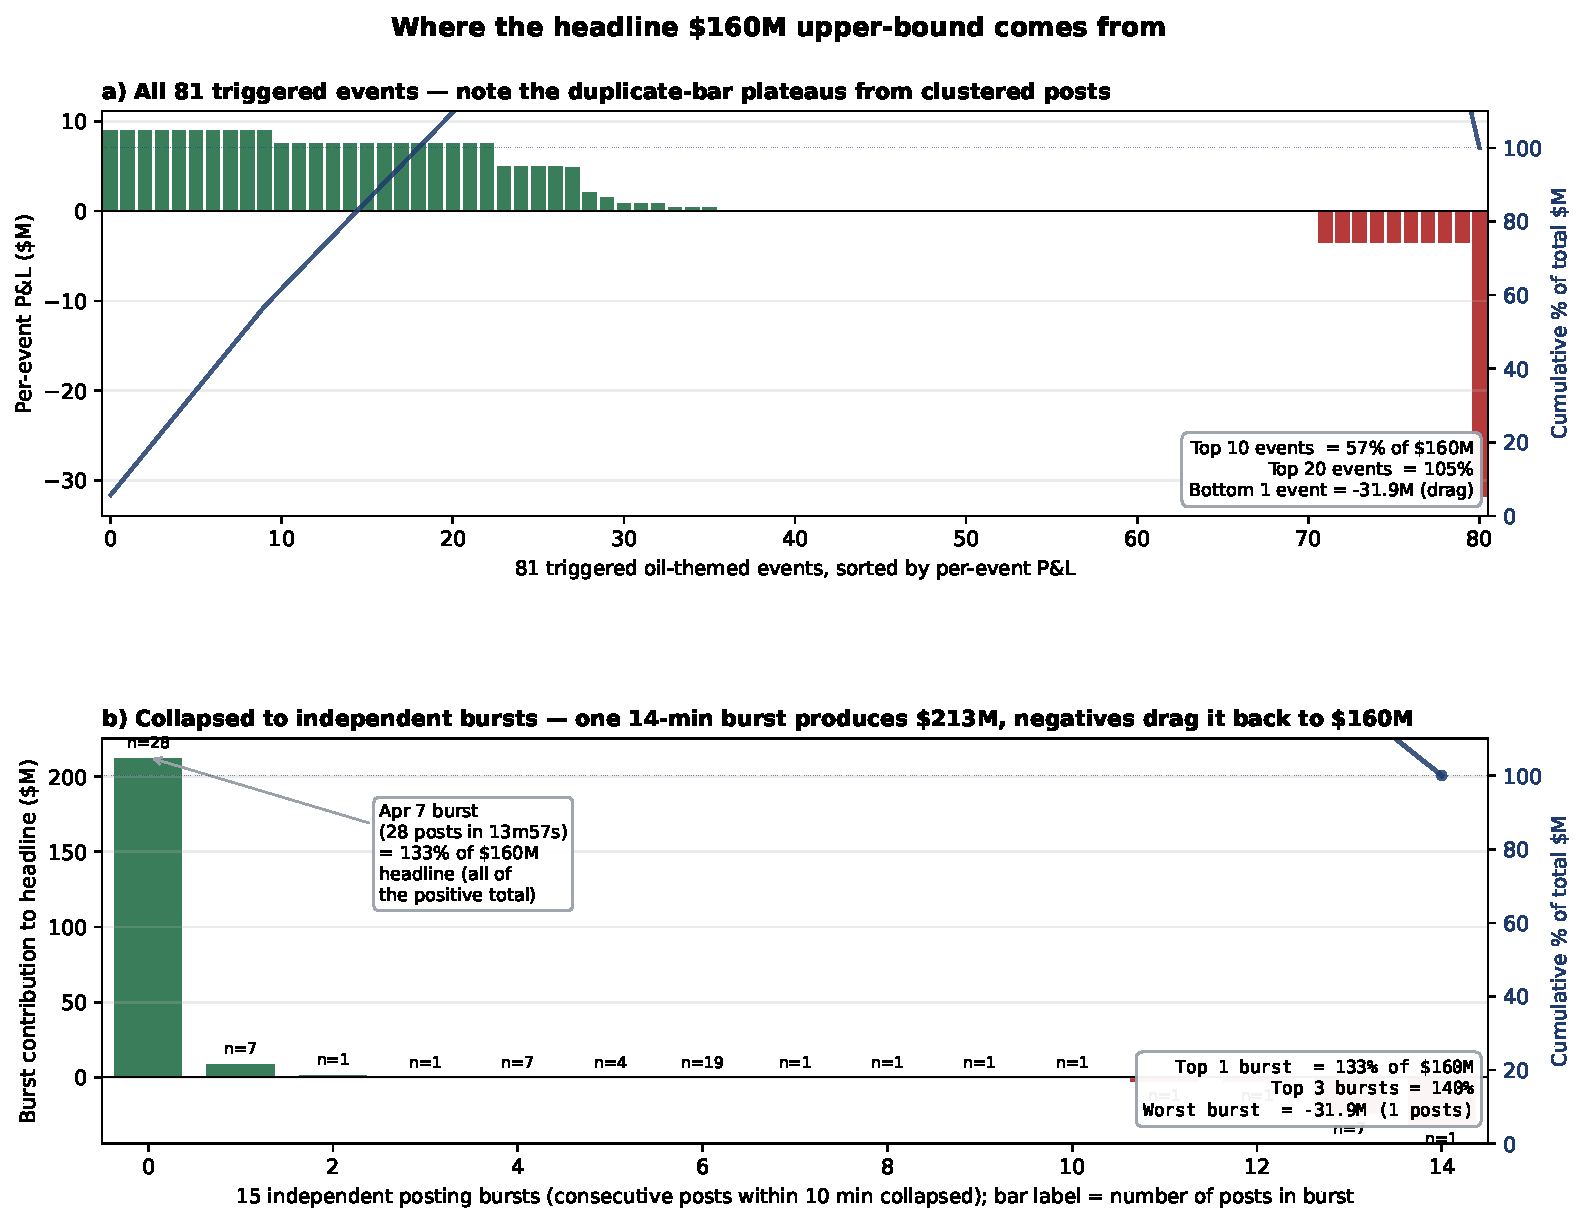
\includegraphics[width=0.98\linewidth]{figures/fig8_pnl_concentration.pdf}
\caption{The same upper bound, viewed by event and by burst. Top panel: per-event P\&L for all 81 triggered events sorted descending; the cumulative line shows that the top 10 events account for $57\%$ of the headline \$160M. Bottom panel: the same events grouped into 15 independent posting bursts (consecutive posts within 10~minutes collapsed). One 14-minute burst on 7~April~2026 (28 posts) contributes \$213M --- essentially the entire positive total --- which negative bursts (chiefly the single 23~March post at $-\$32$M) drag back down to the \$160M headline.}
\label{fig:pnl_concentration}
\end{figure}

This figure is fragile in three specific ways and should be read accordingly.

First, the distribution of per-event P\&L is highly skewed. The median is at or near zero, which means roughly half the events contribute almost nothing. The headline sum is driven by a small number of unusually large events. A single oil-themed post on 23~March~2026 contributes a position-times-move of around $-\$32$~million, or roughly 20\% of the total in absolute terms. Removing that single event swings the headline figure by tens of millions of dollars in either direction. A finding that depends materially on whether one particular event is in or out of the sample is not a robust population statistic.

Second, several oil-themed posts in the window were issued in clusters of near-duplicate text within seconds of each other. On 7~April~2026, four posts landed within a 31-second window; each of them carries an identical pre-event signed-volume measurement and an identical 60-minute forward window, because their pre and post windows are essentially the same window. The arithmetic of our pipeline counts each such post separately, which inflates the aggregate by approximately \$27~million across the four duplicates. Whether or not to dedupe near-simultaneous posts is a methodological choice that materially shifts the headline.

Third, the calculation assumes frictionless execution at bar-close prices, no bid-ask spread, no borrowing cost, no market-impact cost, and no leverage cap. None of these assumptions hold in real trading. A position of the size implied by the cumulative pre-event imbalance would itself have moved the USO price during execution, eroding the gross P\&L. \citet{hasbrouck2009} shows that even daily-data estimators can recover effective trading costs to within a few basis points of the tick-level benchmark, which is the natural starting point for converting a gross figure of this kind into a defensible net figure.

Taken together, these caveats suggest a defensible range for the dollar upper bound somewhere between roughly \$96~million and \$192~million across 81~oil-themed events in the 73-day window, with a single point estimate of \$160~million sitting toward the upper end of that range only under the most permissive assumptions. We strongly resist citing ``\$160~million'' without these caveats. The number is provided to scale the finding in dollar terms; it is not a claim that anyone made this money, nor a regulatory estimate of the size of any actual misconduct.

% ── 6. What the data cannot tell us ──────────────────────────────────────────
\section{What the data cannot tell us}\label{sec:cannot}

A study like this generates more questions than it answers, and several of those questions are louder than the ones we have answered. We address them directly.

\subsection{The signal is consistent with multiple causal mechanisms}

The XLE and USO pre-event signals are correlational. They establish that something unusual is happening in oil trading immediately before Trump posts about oil, and that the something is statistically distinct from matched non-event timestamps and from the same posts shifted by a day. They do not, on their own, establish which of several candidate mechanisms is responsible.

The first candidate is leakage. Someone with advance knowledge of an impending post, or of the intent to post, positions into the relevant instruments before the post lands. This is consistent with the evidence and is the mechanism that would matter most for any regulatory or political conclusion. It is not uniquely identified by our data.

The second candidate is reverse causation on a short horizon. Oil markets move for unrelated reasons, Trump notices the move, and posts in response. The initiated/reactive classifier (Section~\ref{sec:initiated}) addresses this at the two-hour pre-event horizon: only posts where the asset was not already moving over those two hours are included. But we cannot rule out reverse causation on horizons shorter than that, and the 5-minute resolution of our data places a hard floor on what we can observe.

The third candidate is coincident news. A genuine catalyst (a leaked OPEC decision, a geopolitical rumour, an earnings preprint) independently moves oil markets and prompts Trump to post about oil minutes later, with no causal arrow between the two. From price and volume alone, this is impossible to distinguish from leakage. The relevant scholarly literature here is large; \citet{tetlock2007} is the canonical demonstration that media content carries pricing-relevant information beyond what fundamentals alone explain, which means that for any analysis tying social-media posts to subsequent price moves, the possibility that the post and the price are both reading from the same upstream news ticker is a leading hypothesis rather than a footnote. Distinguishing the two would require, for each event, a careful per-post audit of the news wires that hit the tape during the pre-event window. We have not done this, and we flag it as the single most important next step (Section~\ref{sec:future}).

The fourth candidate is residual artefact in the analytical process. The matched placebo and time-shift falsification are designed to minimise this risk, but no statistical procedure eliminates it completely.

We use the phrase ``front-running-consistent pattern'' to describe the signal. We do not use the phrase ``insider trading'', because that phrase requires a specific identified trade by a specific identified person linked to a specific identified post.

\subsection{The named-friends question cannot be answered on this window}

A related question is whether posts that mention specific individuals or companies (Elon Musk, particular Big Tech CEOs, particular Big Oil firms by name, particular Big Banks by name) move the share prices of those entities. This was one of our motivating questions, but the available data does not support an answer on the current window.

The reason is mechanical. Within the 73-day overlap between our minute-level price data and the post archive, Trump posted about Musk or Tesla zero times, about individual Big Oil companies by name zero times, about individual Big Tech CEOs by name once, and about individual Big Banks by name twice. None of these counts come close to the minimum sample size required for a credible event-study cell.

Across the four-year archive as a whole, the named-entity counts are larger (Musk/Tesla 116~posts, Big Tech 43, Big Oil 2, Big Banks 12), but our minute-level data does not extend back far enough to use them. A paid minute-bar feed (Section~\ref{sec:data-needed}) would unlock this analysis on the larger sample. As things stand, we report the named-friends decomposition as a question for future work, not as a finding.

\subsection{We cannot generalise from the oil complex to other sectors}

Our verified findings concern the oil sector specifically: the energy-sector ETF and the crude-oil ETF, around posts about oil. We tested a wider set of instruments and a wider set of topics, and the results outside the oil complex are mixed. Some signals look promising on a single test but fail the time-shift discipline; others are weak. Reporting any of those weaker signals as findings would overstate what the data supports. A reasonable reader should treat the oil findings as a localised result, not as evidence of a generalised pattern across the US equity market. The cross-asset placebo of Section~\ref{sec:crypto-placebo} provides the cleanest available test of the asset-specificity question: order-flow imbalance does not lift on BTC or ETH around the same triggered oil events, which speaks against (though does not exclude) a generic ``Trump moves all risk assets'' interpretation of the OFI signal.

% ── 7. Limitations ───────────────────────────────────────────────────────────
\section{Limitations}\label{sec:limits}

The 73-day window is the binding constraint on most things. A paid minute-bar feed extending two or more years back would materially raise the statistical power available for smaller topics, would unlock the named-friends decomposition (Section~\ref{sec:cannot}), and would allow the time-shift falsification to be run at multiple displacement lengths (one week, one month, one quarter), each of which strengthens the claim that the residual signal is event-aligned rather than seasonal.

Trade direction is inferred, not observed. We do not have access to a tick-level feed that would tell us the buyer-initiated and seller-initiated volume in each bar. The Bulk Volume Classification estimator we use is an approximation that has been shown to agree with true direction on 50--65\% of trades. At the level of statistical aggregates across hundreds of events, this is sufficient to detect real imbalances, but it is not sufficient to attribute any individual trade to any particular agent.

The topic classifier is a regex. We retained it for the reasons given in Section~\ref{sec:data}, but a more sophisticated topic model would likely improve the precision of the topic flag, which in turn would tighten the event-study cells. We expect the direction of any such improvement to strengthen rather than weaken our findings, since a cleaner classifier would push noise out of the test rather than into it.

Posts often arrive in clusters of near-duplicate text within seconds. Our pipeline does not currently dedupe near-simultaneous posts, which is the right choice for the order-flow tests of Section~\ref{sec:findings} (each post is its own discrete event in time) but the wrong choice for the dollar magnitude calculation of Section~\ref{sec:dollars} (where overlapping pre and post windows produce spurious arithmetic inflation). Section~\ref{sec:dollars} reports a range that brackets the dedupe choice; a future iteration of this work should resolve this asymmetry properly.

The 5-minute bars are left-closed, which means a post at 09:33:47 is assigned to the bar labelled 09:30. Up to 4~minutes 59~seconds of misalignment is therefore baked into the event boundary by construction. This blunts any genuinely sub-minute algorithmic effect and is a structural limitation of the data resolution rather than of our pipeline.

% ── 8. Future work ───────────────────────────────────────────────────────────
\section{Future work}\label{sec:future}

We list four extensions in priority order, scoped to what the available evidence most needs.

The most consequential extension is a per-event news-wire audit. For each oil-themed post in the window, we would query a Bloomberg or Reuters news feed for headlines on oil-related stories that hit the tape during the pre-event window. The presence or absence of such headlines bears directly on the coincident-news mechanism in Section~\ref{sec:cannot}. A version of the order-flow finding that conditions on ``no oil news on the tape in the pre-event window'' would substantially narrow the space of plausible explanations.

The second extension is a longer minute-bar window. A historical minute-bar feed from a paid provider such as Polygon.io extending two or more years back would unlock both the named-friends decomposition (Section~\ref{sec:cannot}) and a substantially more powerful time-shift test, as well as letting us test the robustness of the oil-complex finding across a much wider sample of oil-themed posts.

The third extension is a proper deduplication and cluster handling protocol. Posts arriving in clusters of near-duplicates within seconds should be collapsed for the purposes of any aggregate-magnitude calculation, while remaining distinct events for the per-post statistical tests. This is a methodological refinement that materially affects Section~\ref{sec:dollars}.

The fourth extension is a strategy backtest with realistic execution costs. The dollar magnitude in Section~\ref{sec:dollars} is a perfect-foresight upper bound. A version of the finding expressed as a rules-based strategy with bid-ask spread, market impact, and borrow cost would produce a much smaller and much more defensible number. Whatever that number turns out to be, it would be more useful for both reporting and policy purposes than the upper bound we have computed here.

% ── 9. Data required ─────────────────────────────────────────────────────────
\section{Data required to unlock the open questions}\label{sec:data-needed}

Three of the four extensions in Section~\ref{sec:future} cannot be attempted with the data we currently have. This section sets out, in priority order, what data each extension requires, what it costs, and what it would unlock. The aim is to make the next step concrete rather than aspirational, and to give a reader (or a reviewer, or a funder) a clear picture of what a properly resourced version of this work would look like.

\subsection{A historical minute-bar feed extending two or more years back}

The 73-day window is the binding constraint on almost every question we have not been able to answer. Yahoo Finance's free intraday feed is capped at 60~days of 5-minute bars, which is why our overlap with the four-year post archive is only the trailing 73~trading days. A paid feed extending two or more years back would do four things at once.

It would unlock the named-friends decomposition (Section~\ref{sec:cannot}), since the four-year archive contains 116 Musk/Tesla posts, 43 Big Tech posts, 12 Big Banks posts, and a smaller but non-zero count of posts naming individual Big Oil firms, all of which sit outside our current window. It would let us run the time-shift falsification at multiple displacement lengths (a week, a month, a quarter), each of which is an additional independent check that the residual signal is event-aligned rather than seasonal. It would let us run the order-flow tests on a substantially larger sample of oil-themed posts, lowering the floor on what size of effect we can detect. And it would let us test whether the oil-complex pattern is itself stable over multi-year horizons, or whether it has emerged or attenuated within the period of the archive.

The two practical providers are Polygon.io and Databento. Polygon.io's Stocks Advanced tier costs roughly US\$200--400 per month and includes minute aggregates back to 2003 across the full US equity universe. Databento sells historical minute bars on a pay-per-use basis, where a one-shot pull of four years of minute data on the ten ETFs we currently use plus a wider equity universe would cost in the low hundreds of US dollars. Polygon is the better fit if we expect to iterate on the analysis over months; Databento is the better fit for a single bulk download.

\subsection{A news-wire archive with millisecond-stamped headlines}

This is the purchase that addresses the central interpretive ambiguity in Section~\ref{sec:cannot}, which is whether the pre-event signal reflects leakage or coincident news. Without a news-wire feed, we cannot distinguish a world in which someone with foreknowledge of an impending post positions before it lands from a world in which a real catalyst hits the tape and independently moves both the market and Trump. With a news feed timestamped at the same resolution as our market data, we can rerun the order-flow analysis conditional on whether oil-related news hit the tape during the pre-event window. A version of the finding that survives the condition ``no oil news on the wire in the 30~minutes before the post'' would substantially narrow the space of plausible mechanisms, in the direction that matters most for any regulatory or political reading of the result.

Three options at very different price points. The institutional gold standard is a Bloomberg Terminal seat or a Refinitiv/LSEG Eikon subscription, each at roughly US\$25{,}000 per year, both of which return millisecond-stamped headlines that can be queried per-event. The mid-tier option is RavenPack, whose analyst-tagged news feed is the data set most academic finance papers in this area work from; pricing is enterprise-quoted rather than published. The cheapest defensible route is a Benzinga Pro subscription at roughly US\$200--500 per month, whose API provides intraday-stamped headlines with topic tags. For a one-off audit of the 173~oil-themed posts in the current window, a short Benzinga Pro subscription paired with manual cross-checks against archived oil-news sources is the most cost-effective path.

\subsection{Tick-level trade and quote data}

The third data acquisition addresses the BVC approximation discussed in Section~\ref{sec:limits}. With a tick-and-quote feed we no longer need to infer trade direction from price movement, because the data records each individual trade and the bid and offer that prevailed when it executed. This is the data on which the Lee--Ready algorithm operates, and it is what would let us replace BVC with a direct measurement at every step of the pipeline.

NYSE TAQ is the canonical source. Academic users typically access it through Wharton Research Data Services (WRDS), which bundles TAQ into an institutional subscription at roughly US\$10{,}000--30{,}000 per year through a participating university. Databento sells TAQ on a pay-per-use basis at a much lower threshold for a fixed-scope project: a single year of trade-and-quote data on the ten ETFs we currently use is in the low thousands of US dollars. This purchase is third in priority because the placebo and time-shift checks in Section~\ref{sec:findings} already discipline the BVC inference at the population level. Tick data would be necessary for any per-event forensic claim, and would tighten the order-flow signals across the board, but it is not strictly required to defend the findings as currently reported.

\subsection{Short-borrow cost data}

A fourth and smaller item, relevant only if Section~\ref{sec:dollars} evolves from an upper bound into a defensible strategy figure. Realistic execution costs at the size implied by our calculation include the short-borrow rate on the leg of the position that is short USO, particularly during periods of market stress when these rates can be volatile. The two commercial sources are S3 Partners and Markit Securities Finance, both of which sell their data through prime-brokerage relationships rather than as a retail product. Because the strategy backtest is the lowest-priority extension in Section~\ref{sec:future}, this acquisition follows from the others rather than precedes them.

\subsection{Recommended sequencing}

If we had to recommend a single first purchase, it would be one quarter of Polygon.io's Stocks Advanced tier (approximately US\$600--1{,}200 in total). That alone unlocks the named-friends analysis and a much more powerful multi-displacement time-shift design, which between them are the two highest-value extensions in the report. The news-wire purchase follows naturally from there: once the longer minute-bar window has flagged the specific events that warrant a per-event audit, a short Benzinga Pro subscription becomes the right second purchase. Tick-level TAQ data sits in third position, justified only when (or if) the analysis moves from population-level claims to per-event forensic claims. Short-borrow data sits in fourth position, justified only when (or if) the dollar magnitude calculation moves from upper bound to executable strategy.

% ── References ───────────────────────────────────────────────────────────────
\renewcommand{\refname}{References}
\begin{thebibliography}{99}

\bibitem[Benjamini and Hochberg(1995)]{benjamini1995}
Benjamini, Y. and Hochberg, Y. (1995).
Controlling the false discovery rate: a practical and powerful approach to multiple testing.
\emph{Journal of the Royal Statistical Society: Series B (Methodological)}, 57(1), 289--300.

\bibitem[Chakrabarty et~al.(2015)Chakrabarty, Pascual, and Shkilko]{chakrabarty2015}
Chakrabarty, B., Pascual, R., and Shkilko, A. (2015).
Evaluating trade classification algorithms: bulk volume classification versus the tick rule and the Lee--Ready algorithm.
\emph{Journal of Financial Markets}, 25, 52--79.

\bibitem[Easley et~al.(2012)Easley, L\'opez de Prado, and O'Hara]{easley2012}
Easley, D., L\'opez de Prado, M., and O'Hara, M. (2012).
Flow toxicity and liquidity in a high-frequency world.
\emph{Review of Financial Studies}, 25(5), 1457--1493.

\bibitem[Easley et~al.(2016)Easley, L\'opez de Prado, and O'Hara]{easley2016}
Easley, D., L\'opez de Prado, M., and O'Hara, M. (2016).
Discerning information from trade data.
\emph{Journal of Financial Economics}, 120(2), 269--285.

\bibitem[Hasbrouck(2009)]{hasbrouck2009}
Hasbrouck, J. (2009).
Trading costs and returns for U.S. equities: estimating effective costs from daily data.
\emph{Journal of Finance}, 64(3), 1445--1477.

\bibitem[Kyle(1985)]{kyle1985}
Kyle, A.~S. (1985).
Continuous auctions and insider trading.
\emph{Econometrica}, 53(6), 1315--1335.

\bibitem[Lee and Ready(1991)]{leeready1991}
Lee, C. M.~C. and Ready, M.~J. (1991).
Inferring trade direction from intraday data.
\emph{Journal of Finance}, 46(2), 733--746.

\bibitem[MacKinlay(1997)]{mackinlay1997}
MacKinlay, A.~C. (1997).
Event studies in economics and finance.
\emph{Journal of Economic Literature}, 35(1), 13--39.

\bibitem[P\"oppe et~al.(2016)P\"oppe, Moos, and Schiereck]{poppe2016}
P\"oppe, T., Moos, S., and Schiereck, D. (2016).
The sensitivity of VPIN to the choice of trade classification algorithm.
\emph{Journal of Banking \& Finance}, 73, 165--181.

\bibitem[Tetlock(2007)]{tetlock2007}
Tetlock, P.~C. (2007).
Giving content to investor sentiment: the role of media in the stock market.
\emph{Journal of Finance}, 62(3), 1139--1168.

\end{thebibliography}

\end{document}
